%!TEX root = ../Thesis.tex
\chapter{Experimental results}
\label{sec:results}

%--------------------------------------------------------------------------------
\clearpage
\section{Initial investigation: WAFFLE experiment}
\label{sec:waffle}

%The data set and campaign metadata have been published on DTU's data repository (\cite{waffle_dataset}).

As a first step towards assessing the feasibility of the project goals, a short measurement campaign was conducted to gather data for performing exploratory analysis and for investigating the core assumption of advection based flow transport.

Work contained in this chapter is expanded upon a poster presentation given at the 3rd International Conference on Future Technologies in Wind Energy (WindTech 2017 in Boulder, Colorado).

A 3-week field experiment named 'WAFFLE' took place between March 23rd and April 6th, 2017 at DTU-Ris{\o} campus. A single long-range scanning lidar (Leosphere WindCube 400S) was deployed at ground level in the field of DTU's research wind turbines. 

The lidar was set to perform scans facing west to measure the dominant wind inflow to the test site. A PPI (sector scan) configuration was used with a sampling rate of 23 seconds, maximum range of 9.6 km, and scanning elevation of 3 degrees (see depiction in Figure \ref{fig:waffle_experiment_setup}).

The dataset has been made publicly available in DTU's data repository (\cite{waffle_dataset}) and a subset was also utilized in an applied workshop with data and code examples available in \cite{simon_eawe_workshop}.

\begin{figure}[htbp]
    \centering
        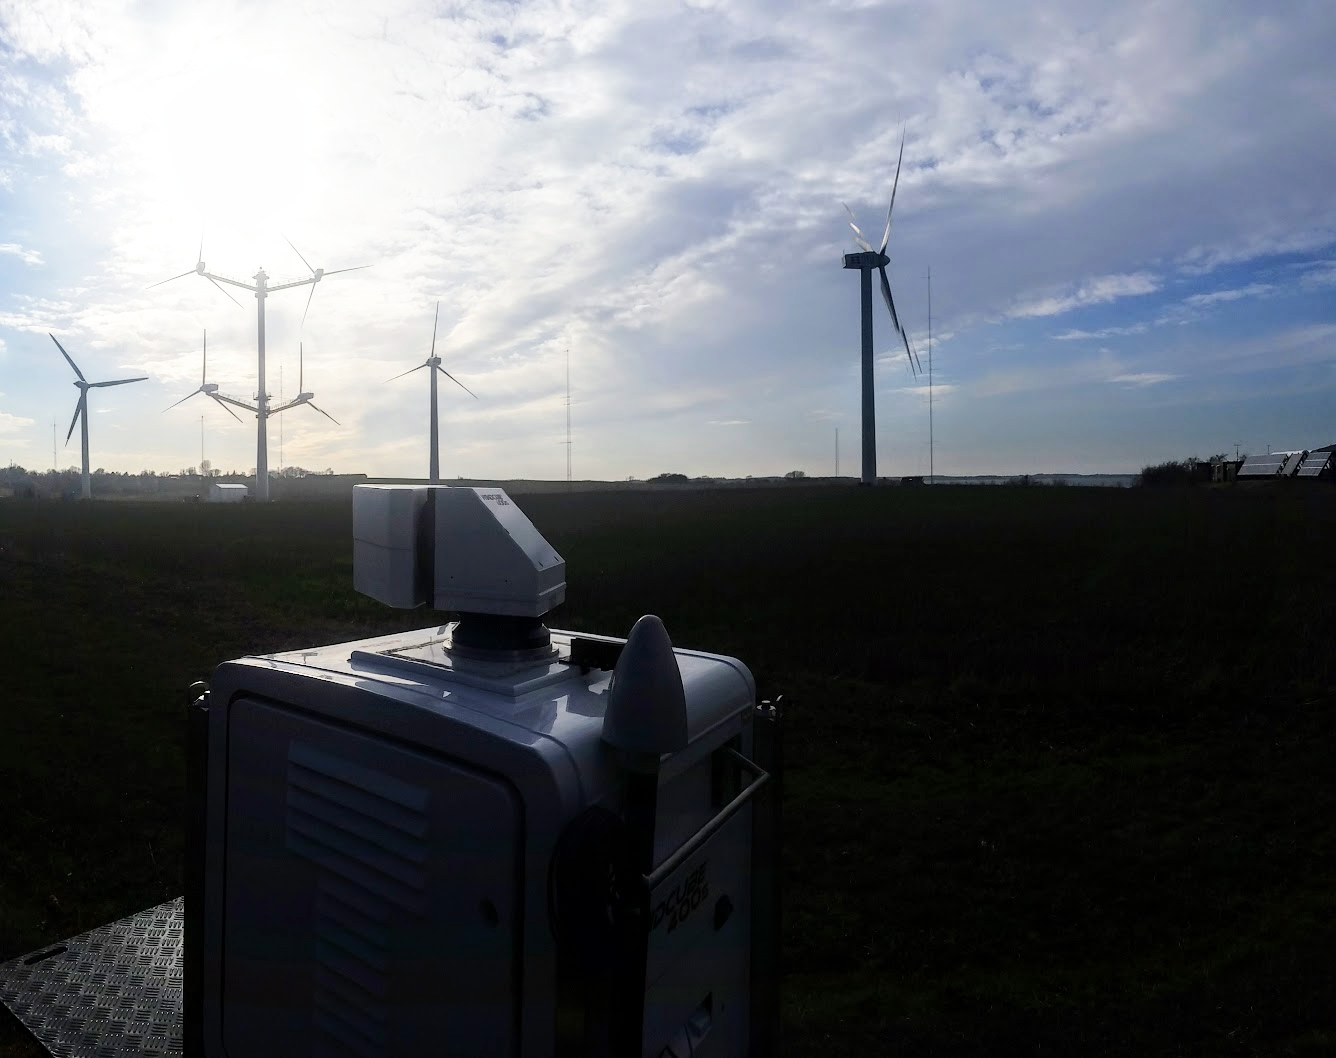
\includegraphics[width=0.465\textwidth]{graphics/results/waffle/waffle_field_photo.png}        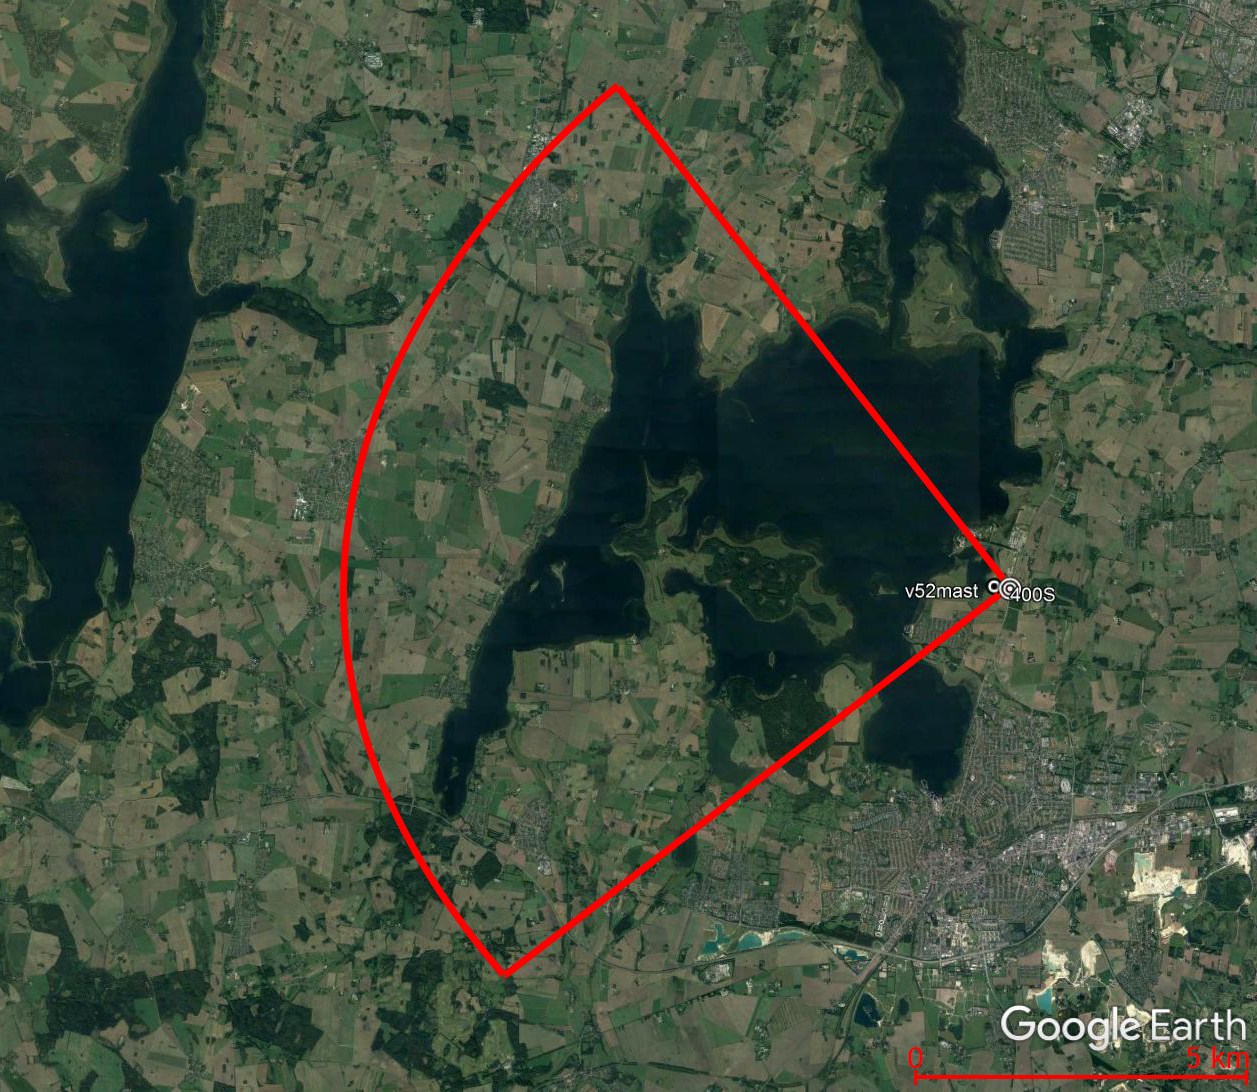
\includegraphics[width=0.43\textwidth]{graphics/results/waffle/experiment_overview_crop.png}
    \caption{Left: Photo of scanning lidar taken during experiment. Right: Aerial view of measurement setup}
    \label{fig:waffle_experiment_setup}
\end{figure}

The elevation angle was necessary in order for the beam to clear the vegetation and other infrastructure present at the site. This however, resulted in a height change as a function of range at a relationship of 52 meters per kilometer. During the data analysis stage, it was determined that this elevation gradient caused a significant issue, both due to the probe volume averaging being affected by wind shear and the lack of correlation of winds at higher heights- the furthest range gate (9.6 km) being at 500 m AGL while the first (288 m) corresponding to 15 m AGL. 

A rudimentary but accepted method to normalize the height differences was applied using the wind profile power law. This is a simple engineering model based on empirical relationships between wind speeds at two heights. During periods of neutral atmospheric conditions, this approach has been well demonstrated to perform similarly to the logarithmic wind profile law above the surface layer and up to the height of the boundary layer <add ref>.

\begin{equation}
    \centering
        u = u_{r} \left( \frac {z} {z_{r}} \right) ^ {\alpha}
    \label{eq:wind_power_law}
\end{equation}

Where $u$ and $z$ are the target wind speed and height, $u_r$ and $z_r$ are the reference wind speed and height, and $\alpha$ is an empirically derived coefficient, often given as 1/7 $\approx$ 0.143 for neutral atmospheric stability.

A 2-day period with westerly winds and neutral/near-neutral stability was chosen and two range gates (RG) were selected which were spaced reasonably far apart but within a range of heights relevant for wind energy purposes. Measurements at the 1200 m RG distance (62 m AGL) and the 1800 m RG distance (93 m AGL) were reconstructed into horizontal wind vector components using the IVAP (integrating velocity azimuth process) algorithm from \cite{liang_ivap_2007} which are given in Equations \ref{eq:ivap_equation_u} and \ref{eq:ivap_equation_v}. From there, the scalar horizontal wind speeds and directions were obtained (Equations \ref{eq:wsp} and \ref{eq:wdir}).

\begin{equation}
    u = \frac{\sum_{\theta_{start}}^{\theta_{stop}} (U_r*\cos \theta ) * \sum_{\theta_{start}}^{\theta_{stop}} (\sin^2 \theta )- \sum_{\theta_{start}}^{\theta_{stop}} (U_r*\sin \theta ) * \sum_{\theta_{start}}^{\theta_{stop}} (\cos \theta  * \sin \theta )}
    {\sum_{\theta_{start}}^{\theta_{stop}} (\cos^2 \theta )*\sum_{\theta_{start}}^{\theta_{stop}} \sin^2 \theta  ) - \sum_{\theta_{start}}^{\theta_{stop}} (\cos \theta  * \sin \theta )^2}
    \label{eq:ivap_equation_u}
\end{equation}

\begin{equation}
    v = \frac{\sum_{\theta_{start}}^{\theta_{stop}} (U_r*\sin \theta ) * \sum_{\theta_{start}}^{\theta_{stop}} (\cos^2 \theta )-\sum_{\theta_{start}}^{\theta_{stop}} (U_r*\cos \theta ) * \sum_{\theta_{start}}^{\theta_{stop}} (\cos \theta  * \sin \theta )}
    {\sum_{\theta_{start}}^{\theta_{stop}} (\cos^2 \theta )*\sum_{\theta_{start}}^{\theta_{stop}} (\sin^2 \theta ) - \sum_{\theta_{start}}^{\theta_{stop}} (\cos \theta  * \sin \theta )^2}
    \label{eq:ivap_equation_v}
\end{equation}

\begin{equation}
    U_h = \sqrt{u^2 + v^2}
    \label{eq:wsp}
\end{equation}

\begin{equation}
    \psi = arctan2\: (v,u)
    \label{eq:wdir}
\end{equation}

Where $\theta$ are the range of azimuth angles of the PPI scan, $U_r$ are the corresponding radial velocity measurements, $U_h$ is the scalar horizontal wind speed, and $\psi$ is the wind direction.

Measurements spanning April 7-8 (7226 23-second samples or approximately 46 hours) were used for the following investigation. The methods utilize reconstructed lidar data at two positions which have been height corrected to 93 m AGL relative to the lidar's telescope: The further upwind position (1800 m RG), and the closer downwind position (1200 m RG). The downwind position is treated as a reference, and three forecasting methods have been performed.

The lead time for the forecasts was set at 70-seconds. This is derived from the theoretical mean advection time by considering the average wind speed (8.55 m/s) during the period together with the horizontal travel distance between the two points (600 m). 

The first method is a persistence benchmark, which simply assumes that the wind speed will remain unchanged over the forecast horizon from the last available measurement. For this, only the reference signal is used (i.e. not the upwind measurements).

The second method, called 'scan-shifting', uses measurements at the upwind position (with no additional modelling) from the current time to predict wind speeds for the downwind position at a given time in the future (current time + forecast length). As the scan rate of the lidar is fixed at 23-seconds, a shift of 3 scans (69-seconds) was used to match the chosen forecast length.

A demonstration of the scan-shift method is shown in Figure \ref{fig:waffle_scan_shift_example} from April 8th of the WAFFLE experiment. When comparing the two signals in real time, a phase error is apparent. After shifting the upwind signal as a function of scan-times, the signals converge to a large degree.

\begin{figure}[htbp]
    \centering
        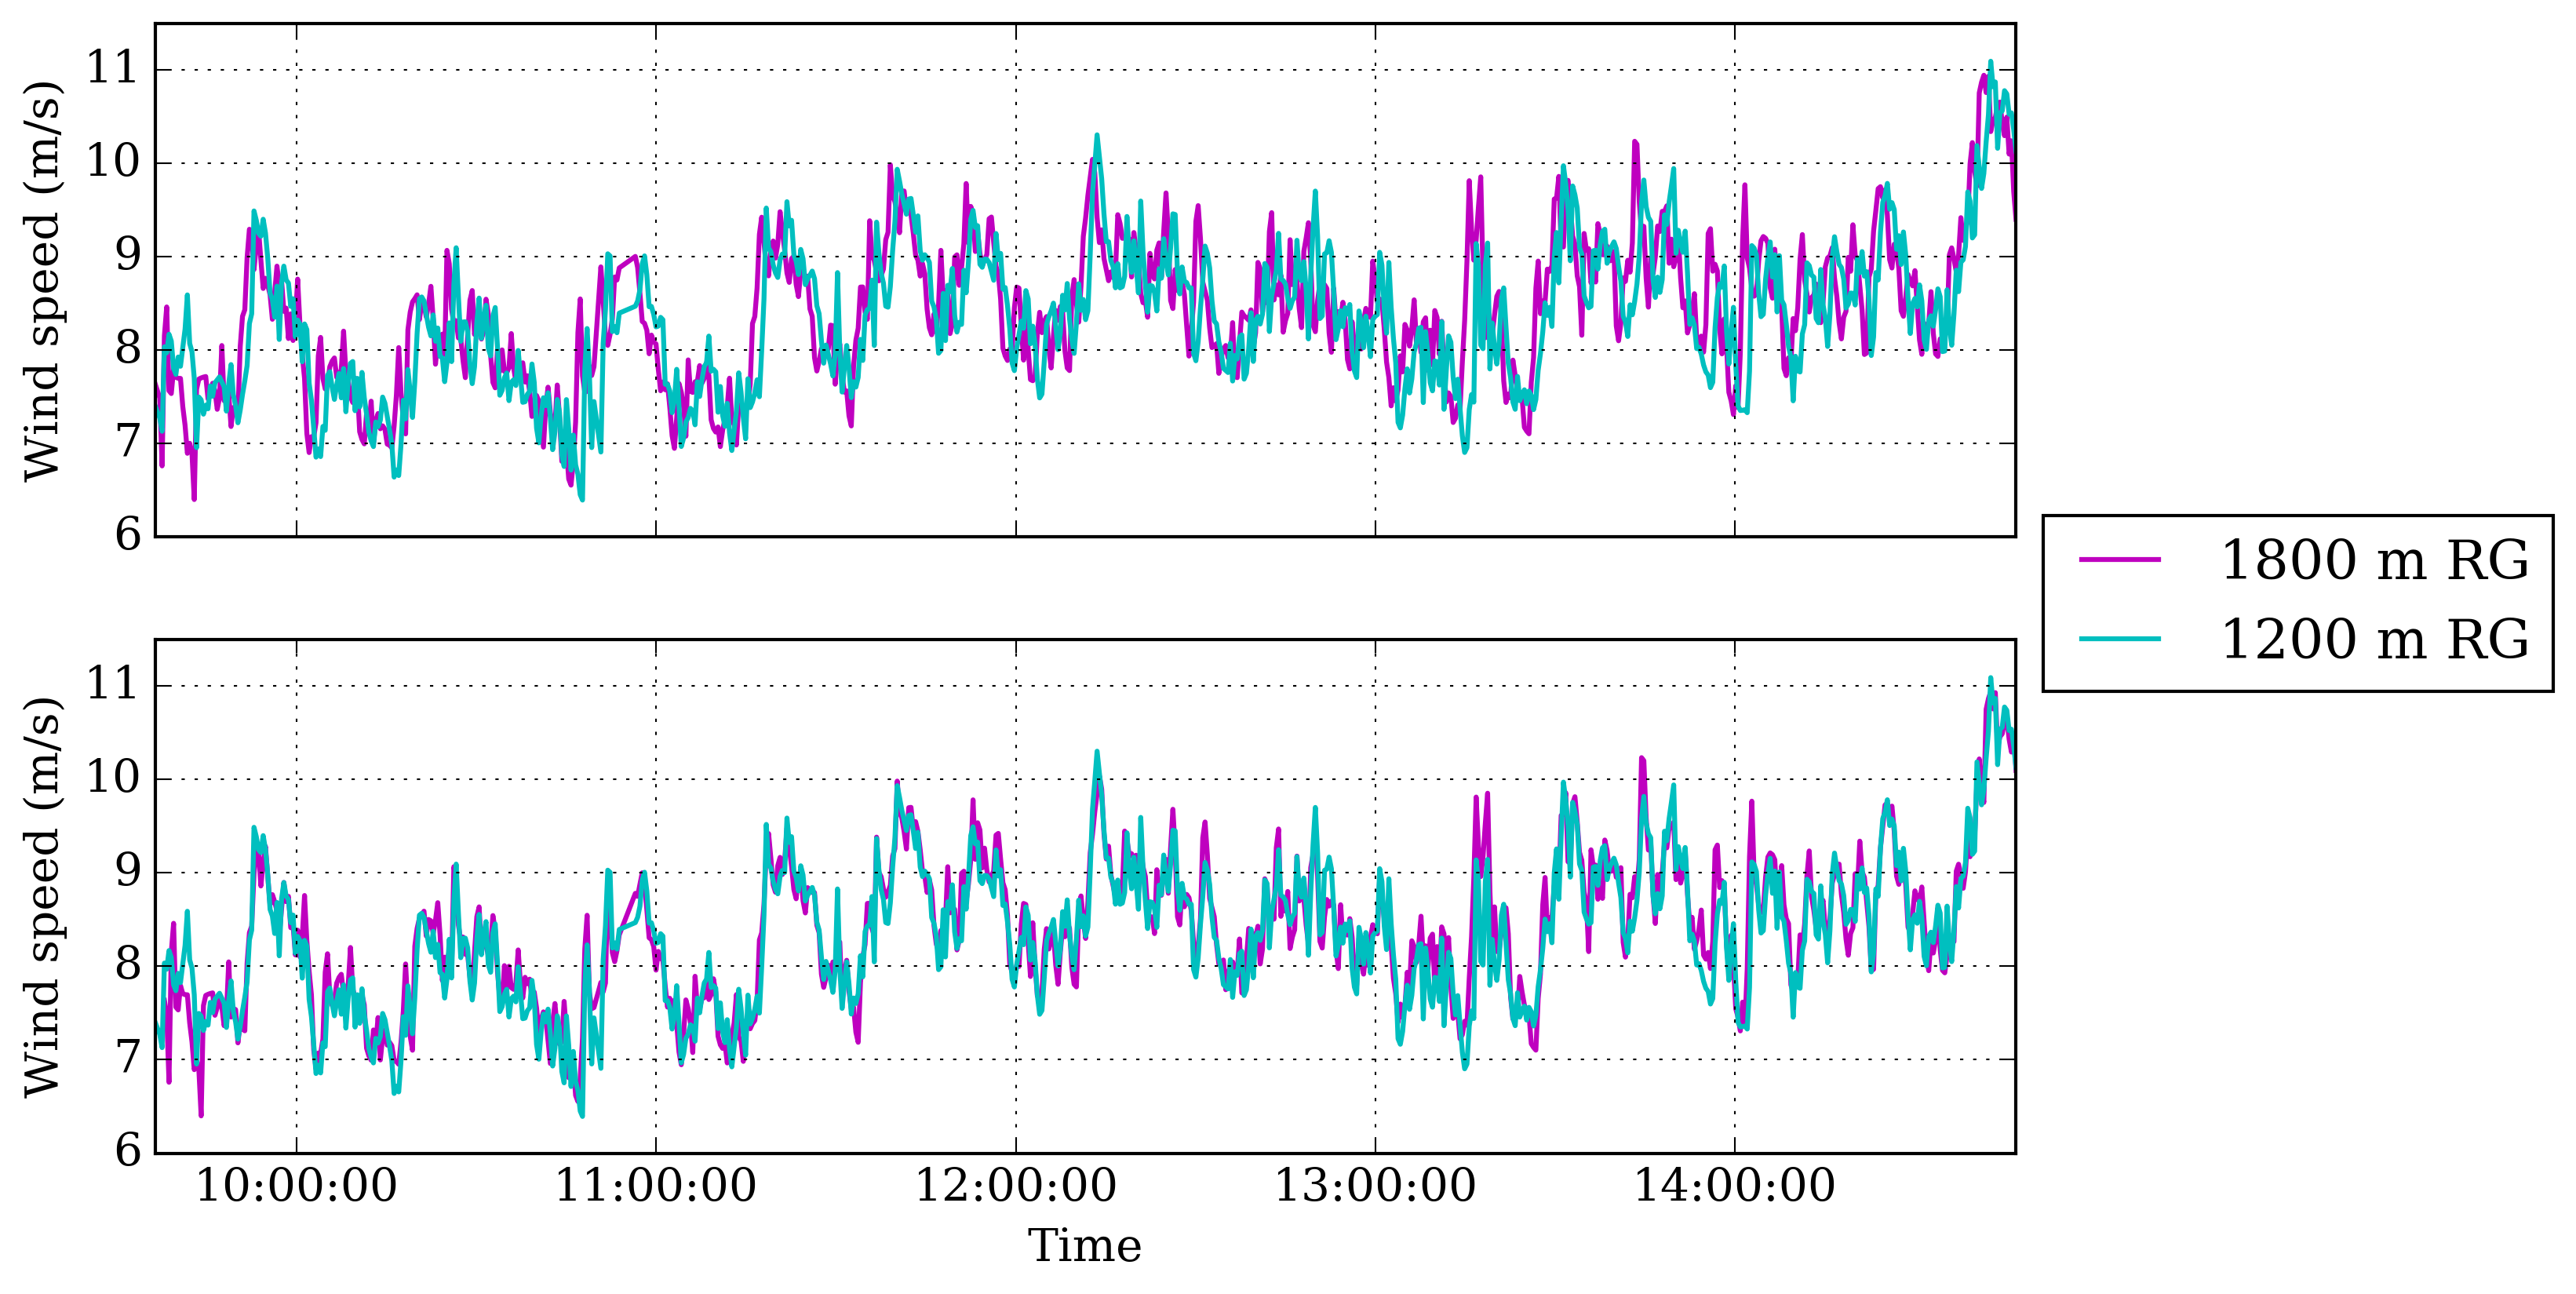
\includegraphics[width=1.0\textwidth]{graphics/results/waffle/waffle_scan_shift_example.png}
    \caption{Time series example of the scan-shift method. Top: Reconstructed wind speeds at the two range gates in real time. Bottom: Upwind signal shifted by 3 scan-times to demonstrate agreement with downwind signal}
    \label{fig:waffle_scan_shift_example}
\end{figure}

As an further sanity check of the scan-shift method, upwind measurements were shifted by a range of scan-times and cross-correlated with the reference values to determine if a peak is present at the number of scans corresponding to our mean advection rate and chosen forecast length. Figure \ref{fig:waffle_1200_shifted1800_corrplot} shows this result, where a clear correlation peak can be seen at the number of scan-times corresponding with the theoretical position.

\begin{figure}[htbp]
    \centering
        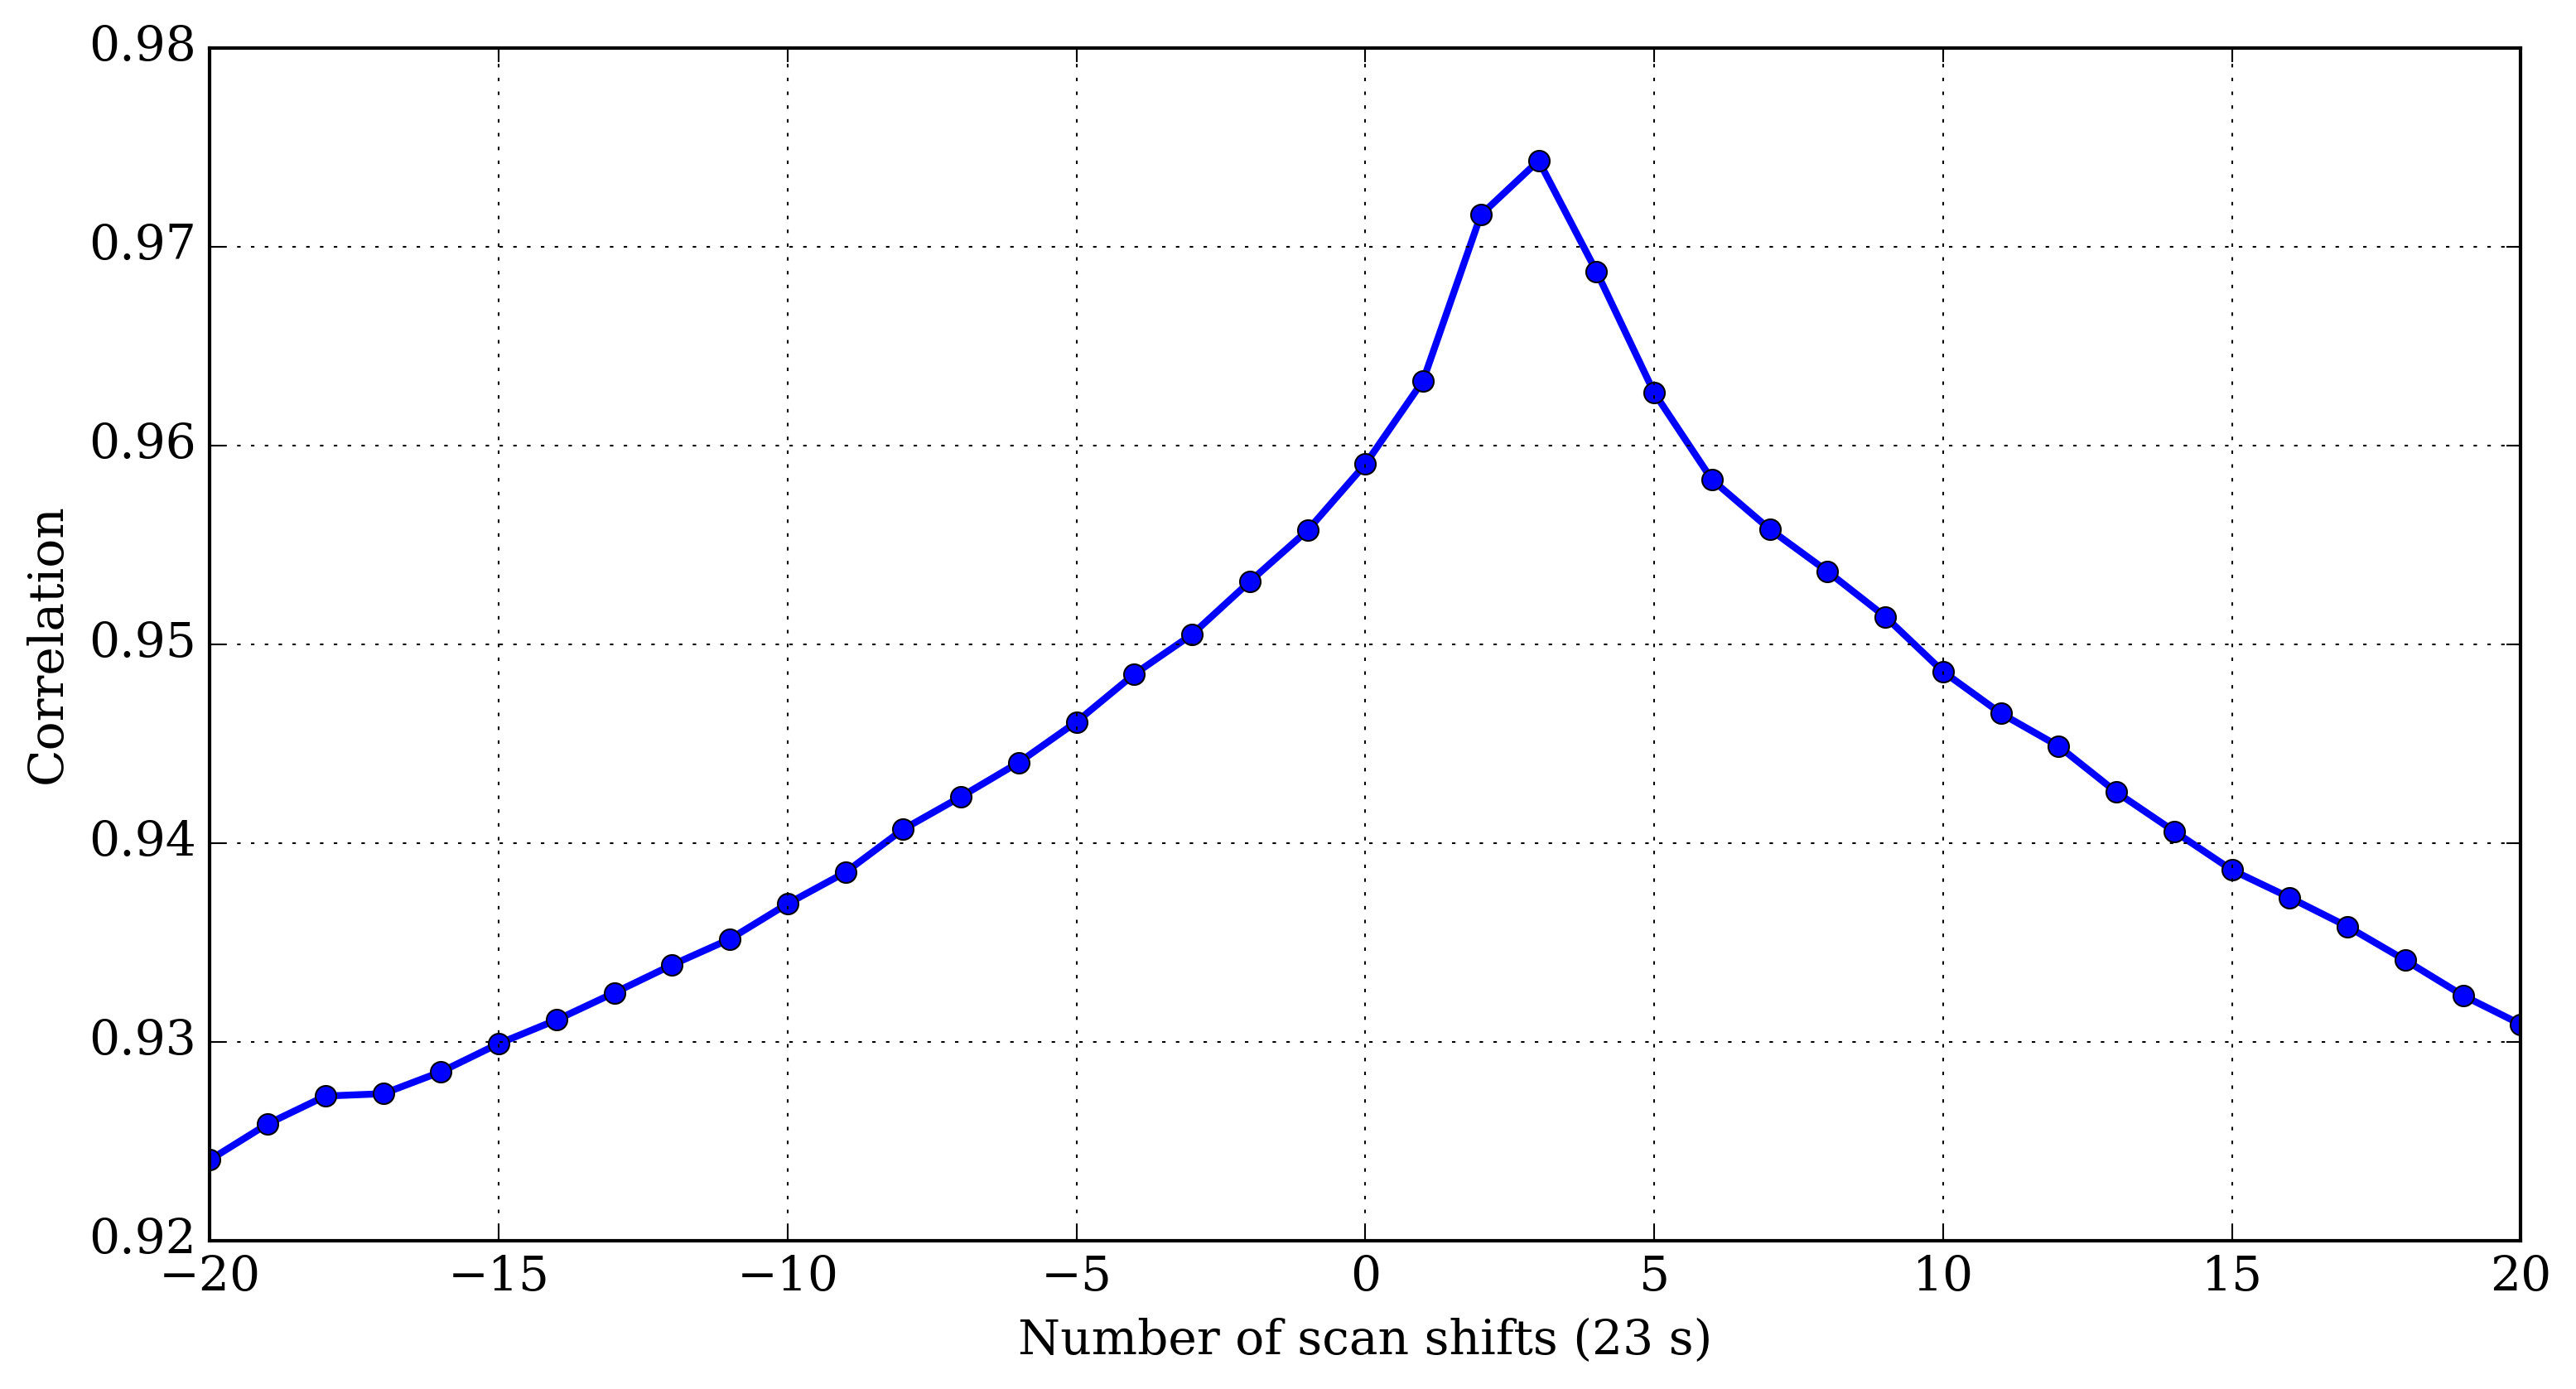
\includegraphics[width=0.7\textwidth]{graphics/results/waffle/waffle_1200_shifted1800_corrplot.png}
    \caption{Cross-correlation function for a range of scan-shifts between the upwind and downwind measurements. A peak exists at the expected location corresponding to the mean advection time}
    \label{fig:waffle_1200_shifted1800_corrplot}
\end{figure}

The final method constitutes building a regression model which takes the upwind measurements as an input to predict the downwind wind speed at the same forecast length. As the number of samples is small, the support vector regression (SVR) method from \cite{drucker_svr_1996} with radial basis function (RBF) kernel was used. This was implemented using the scikit-learn library using default settings and without parameter tuning (\cite{sklearn_svr_docs}). The model was trained on 40\% of the available data and once fitted, was used to make predictions over the entire dataset, as to produce the same sample size as the other methods.

In addition to evaluating forecast performance on wind speeds, a transformation to wind power was made using a power curve model (Figure \ref{fig:waffle_power_curve}). This illustrates a generic turbine model where units are expressed such that a value of one represents the wind turbine generator's rated power. The nonlinear power curve perverts forecast error impacts at different wind speeds, so it is pertinent to also inspect errors in the power domain.

\begin{figure}[htbp]
    \centering
        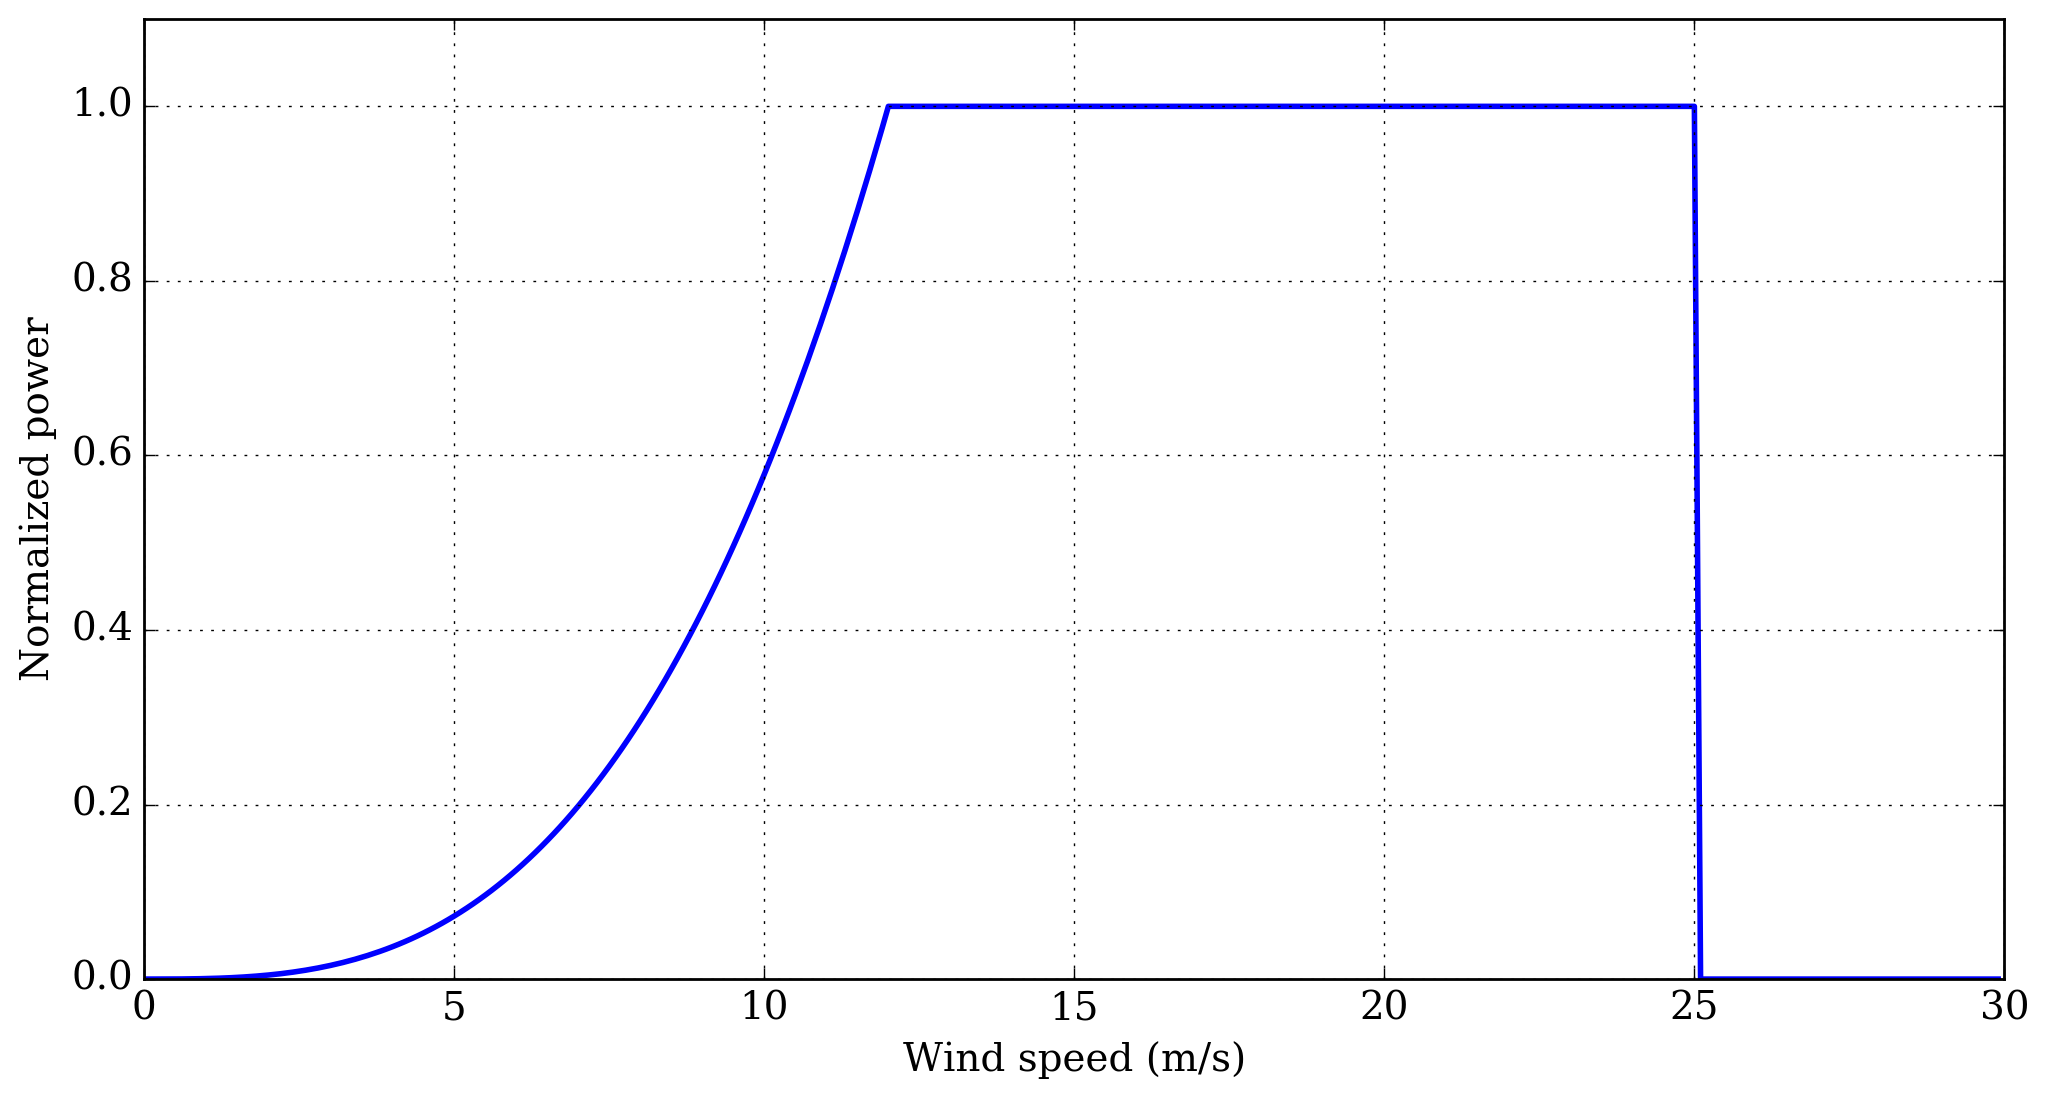
\includegraphics[width=0.7\textwidth]{graphics/results/waffle/power_curve.png}
    \caption{Power curve of generic wind turbine. Normalized such that a value of one represents the turbine's full rated power}
    \label{fig:waffle_power_curve}
\end{figure}

An overall results comparison of the three methods is presented in Figure \ref{fig:waffle_forecast_all_results}, both for wind speed and wind power. The two lidar approaches have improved significantly over the persistence method, with a reduction in root-mean-squared-errors (RMSE) of 20\% for wind speed and 30\% for wind power. Persistence performs well at very low wind speeds (below 5 m/s), but displays larger amounts of scatter exceeding this. There does not appear to be a marked difference in performance between the scan-shift and SVR methods.

\begin{figure}[htbp]
    \centering
        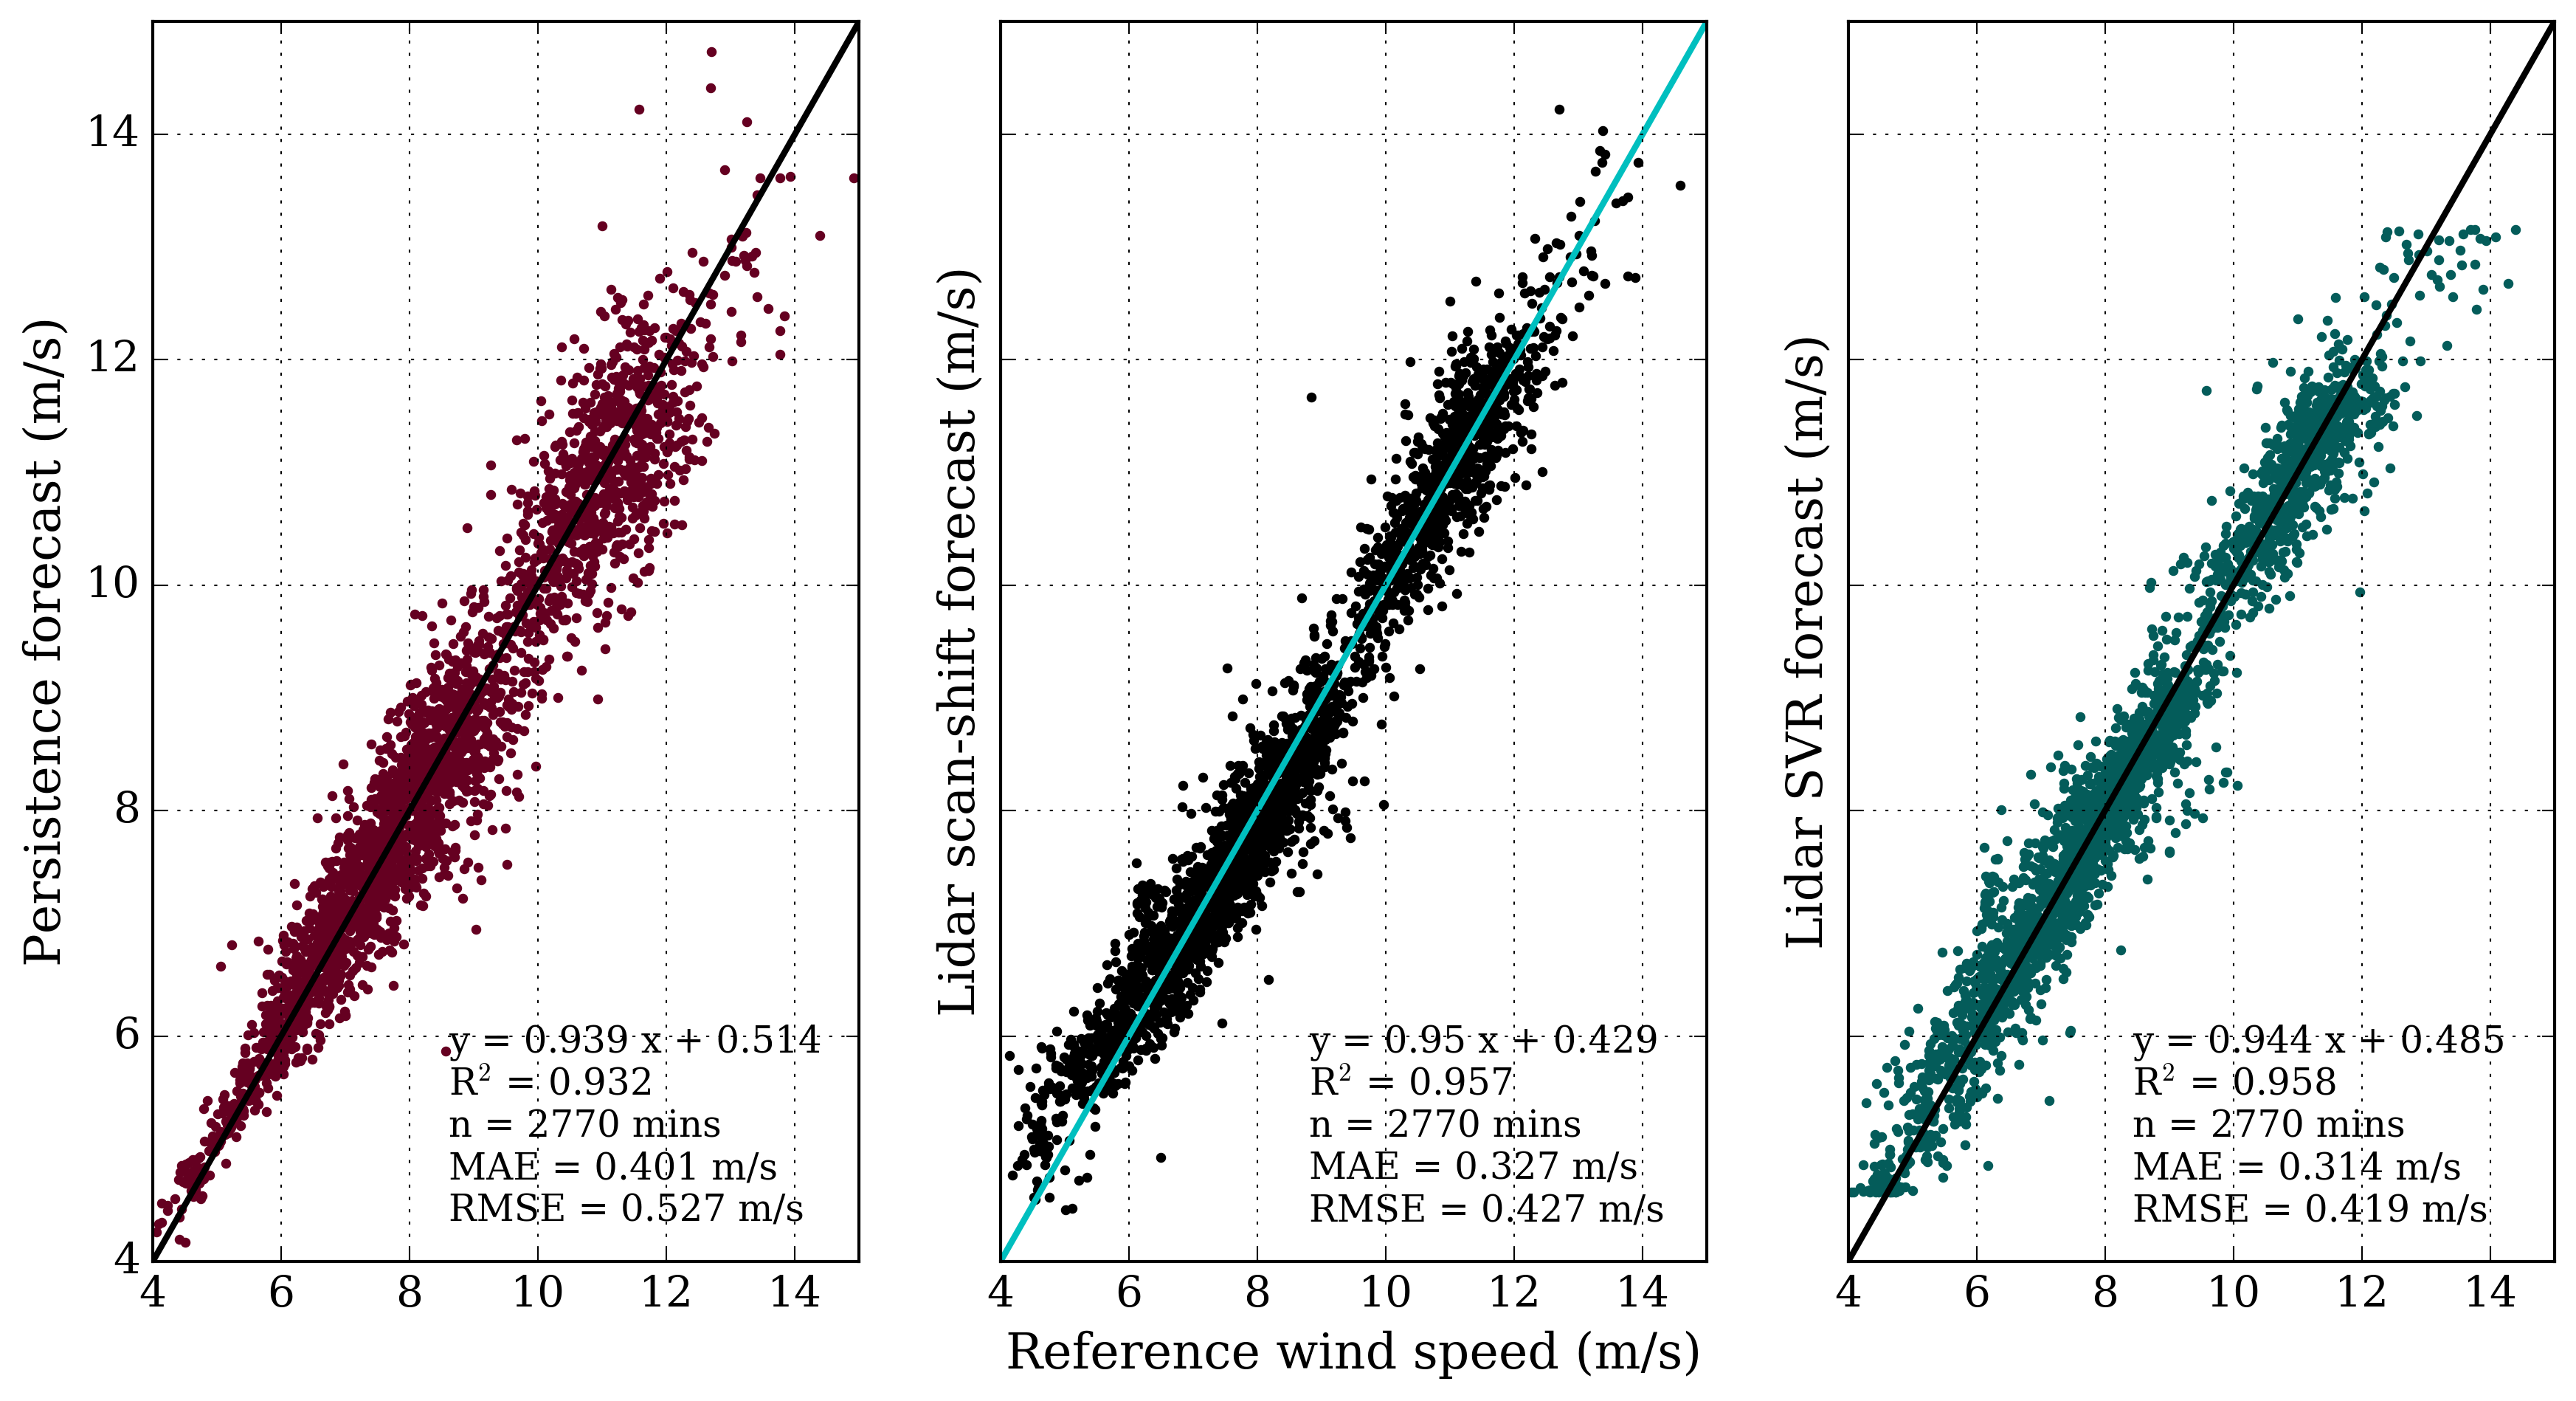
\includegraphics[width=1.0\textwidth]{graphics/results/waffle/waffle_forecast_all_results.png}
        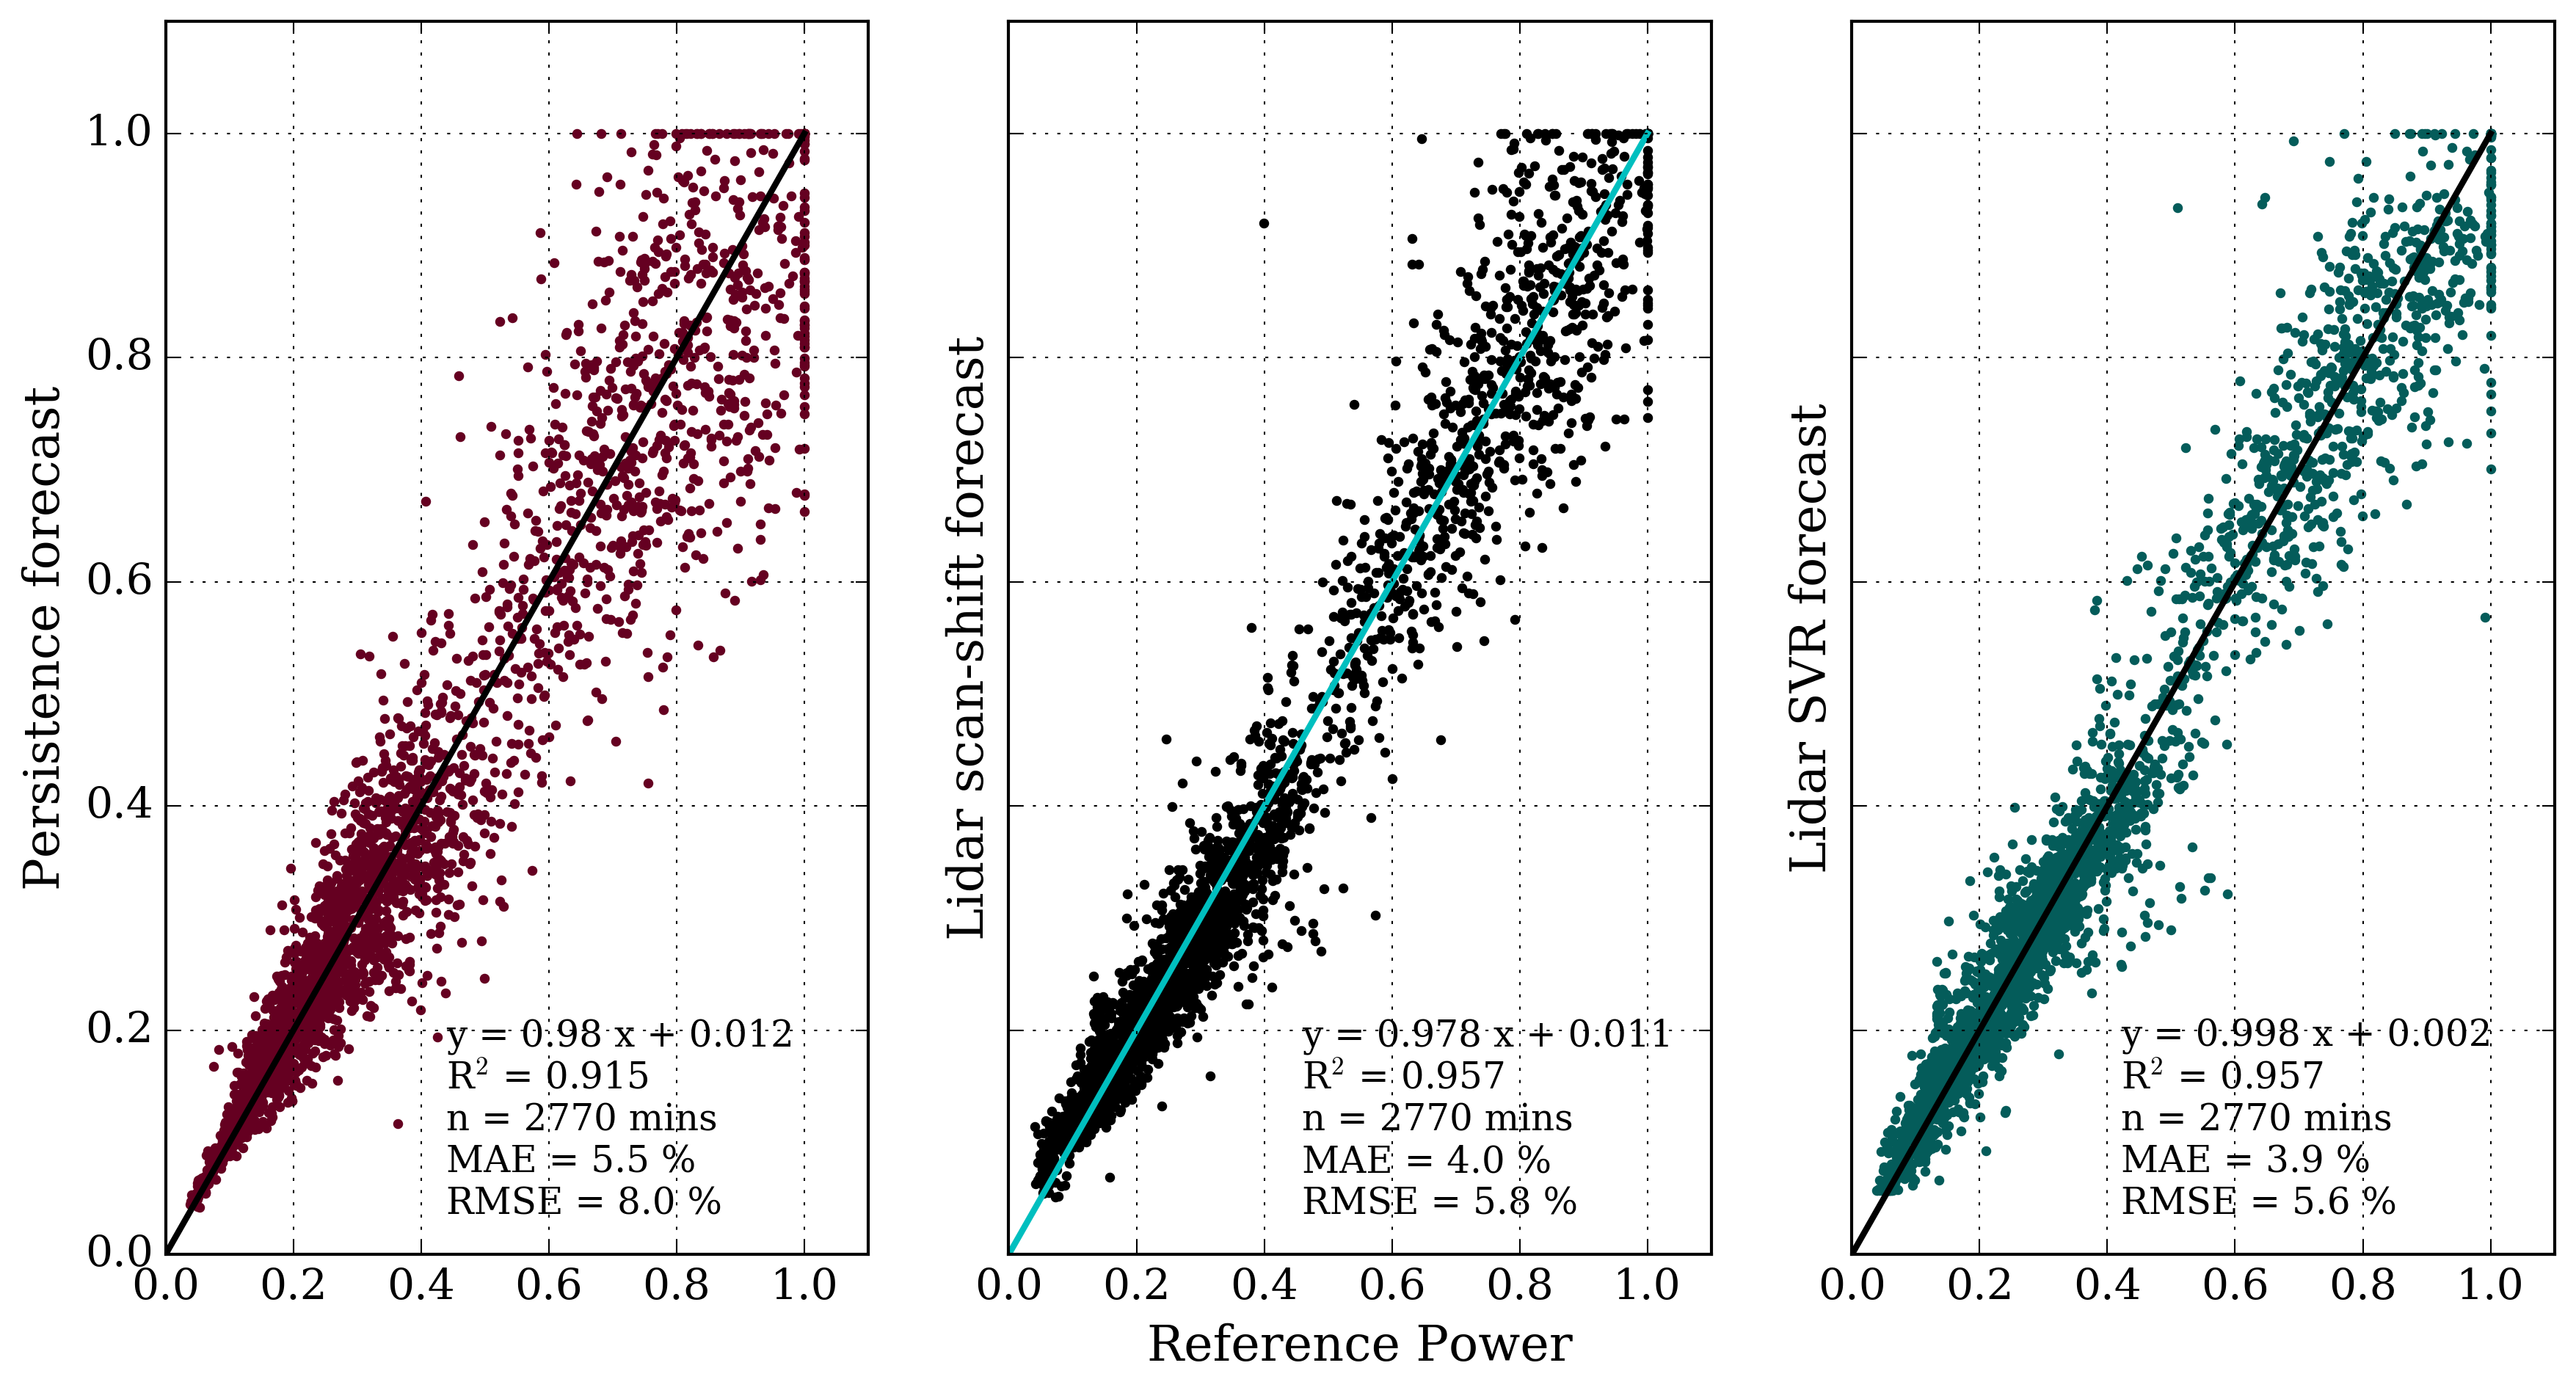
\includegraphics[width=1.0\textwidth]{graphics/results/waffle/waffle_forecast_all_power_results.png}
    \caption{Comparison of three approaches with line y=x also shown. General linear model fit parameters and error metrics annotated}
    \label{fig:waffle_forecast_all_results}
\end{figure}

In summary, two novel forecasting methods have been applied using upwind lidar measurements to generate 1-minute ahead wind speed and power forecasts which significantly outperform the persistence benchmarks. The promising results achieved promote further development of the concept. Adjustments to the measurement setup are strongly recommended in future field campaigns, in order to avoid issues arising from sampling horizontal winds across a sloped plane.

%--------------------------------------------------------------------------------
\clearpage
\section{Addendum: Key results and lessons learned}
\label{sec:waffle_addendum}

\bigskip

\begin{itemize}
    \item A short pilot experiment was carried out to investigate the use of upwind lidar measurements for minute-scale forecasting.
    \item The inclined measurement plane resulted in difficulties relating positions that were spaced kilometers apart due to the height difference between range gates.
    \item The empirical space-time correlation function between upwind and downwind measurements matched well to the theoretical approximation using the mean speed advection of the horizontal winds.
    \item Two novel forecasting methods using upwind lidar measurements were implemented to predict 1-minute ahead wind speeds at the downwind reference position. A persistence benchmark was also performed.
    \item The two lidar methods have demonstrated superior performance against the persistence benchmark, with similar error metrics between each other (both reducing RMSE wind speed errors by 20\%).
    \item Forecast performance has also been evaluated in the wind power domain by applying a wind turbine power curve model. The lidar methods have also outperformed the benchmark by a 30\% reduction in RMSE.
\end{itemize}

%--------------------------------------------------------------------------------
\clearpage
\section{Introduction to second study: 
{\O}sterild Balconies experiment}
\label{sec:balcony_intro}

Building upon the methods and results of the initial investigation, a full scale experiment was planned in conjunction with the New European Wind Atlas (NEWA) project. A primary objective of the campaign was to collect data for the purpose of developing a minute-scale wind forecasting system using upwind observations from the scanning lidars. The resulting {\O}sterild Balconies experiment provides cross-sectional scans of the horizontal wind by performing PPI scans at a height raised above the ground. This avoids the wind shear and height difference problems revealed in the initial investigation.

\noindent
An in-depth report of the experiment and research results are presented in the open access journal article Section \ref{sec:balcony_paper}, which is expanded upon in Addendum 1 (Section \ref{sec:balcony_addendum1}).

\noindent
The data set and campaign metadata have been published on DTU's data repository (\cite{balcony_dataset}).

%--------------------------------------------------------------------------------
\clearpage
\section{Minute-Scale Wind Speed Forecasting Using Scanning Lidar Inflow Measurements}
\label{sec:balcony_paper}

%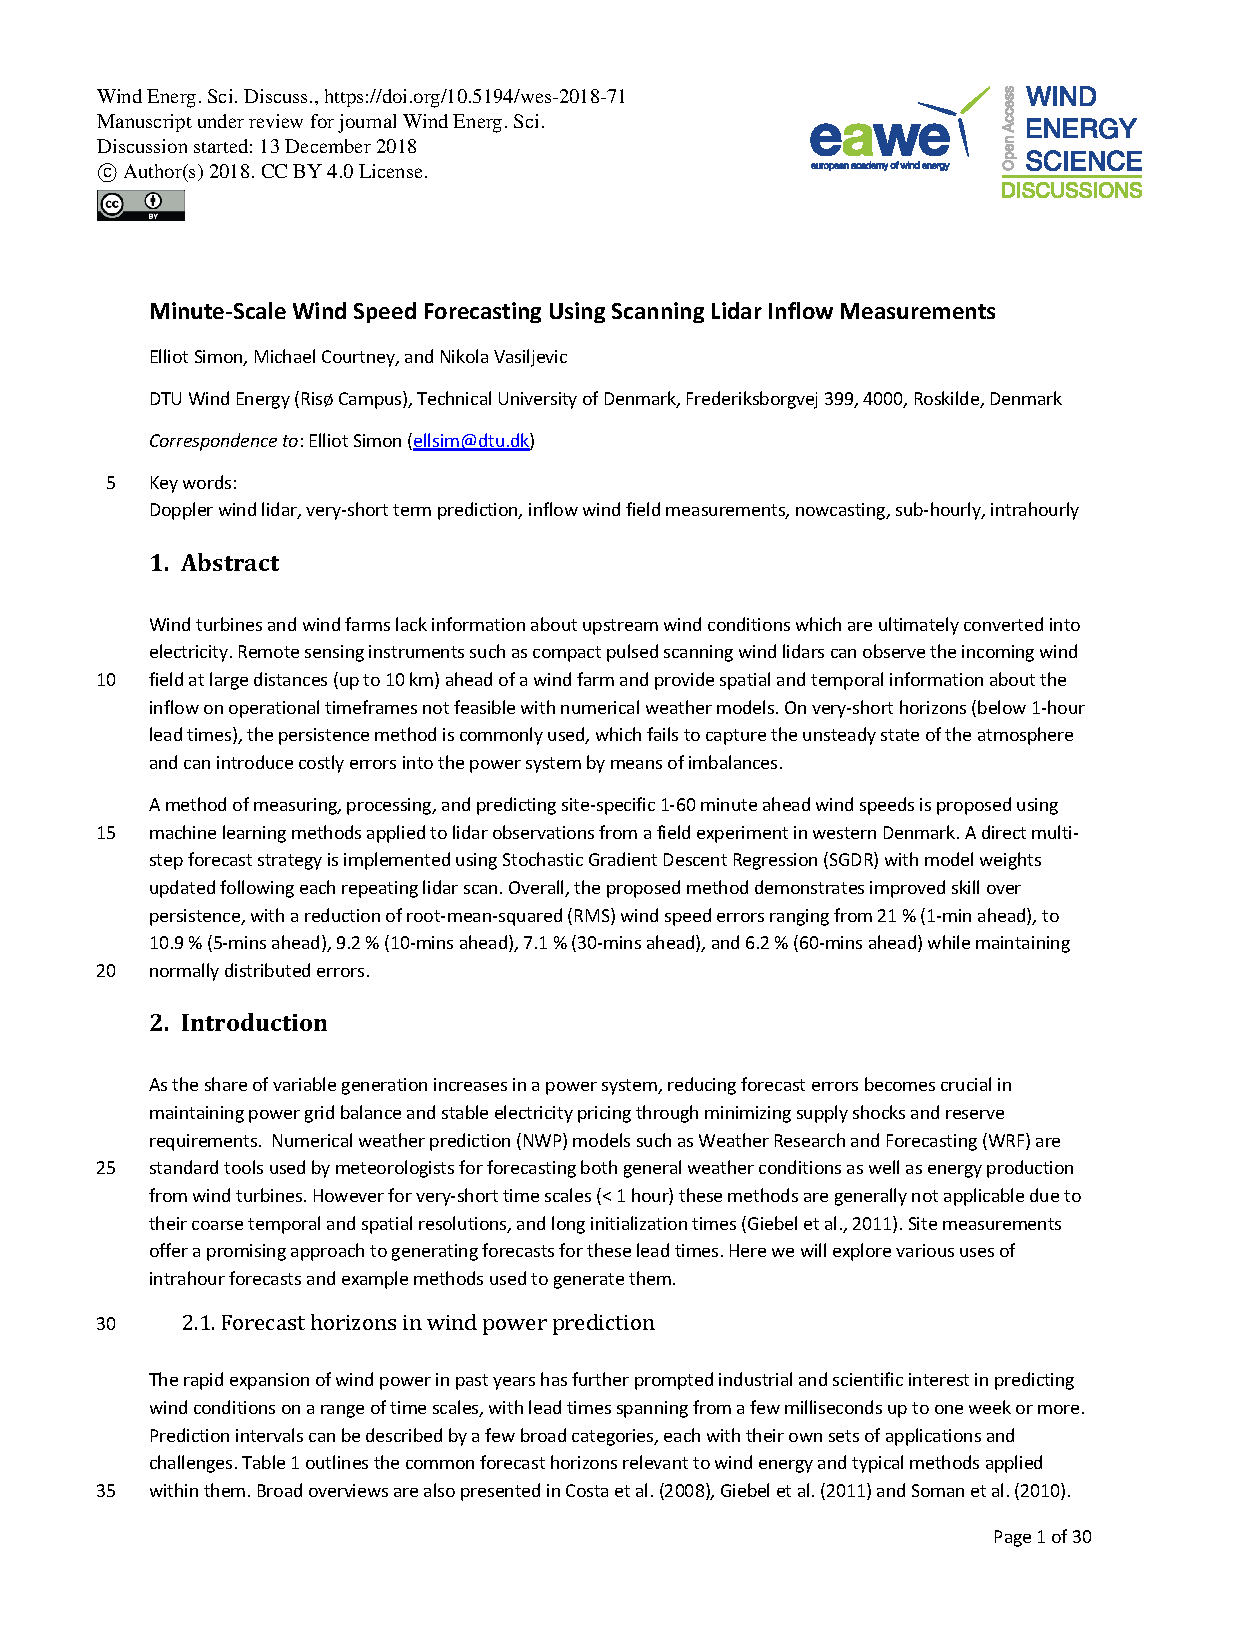
\includepdf[pages=-]{papers/Balcony_paper_WESD.pdf}

%--------------------------------------------------------------------------------
\clearpage
\section{Addendum 1: Weather front case study}
\label{sec:balcony_addendum1}

This section expands upon an oral presentation titled "Lidars Lifted: The {\O}sterild Balconies Experiment" given at the 97th American Meteorological Society (AMS) conference in Seattle (\cite{simon_lidars_lifted_2017}).

During the first phase of the Balconies experiment while the scanning lidars were deployed at 50 m above ground level (AGL),
a weather event was encountered with a potentially high impact for an operational wind turbine or wind farm.

At approximately 6PM UTC on the 6th of June 2016, the arrival of a cold front drastically changed the wind regime at the test site. Although it did not cause a significant wind speed ramp, the wind directions of the two air masses were diametrically opposed. The result was a near instant 180 degree shift in wind direction (from 130 to 310 degrees) as the frontal advection displaced the formerly presiding conditions. 

This example of sudden and extreme veer has undesired and potentially damaging effects for a wind turbine. From an energy production perspective by requiring significant time and control adjustments to adapt to the new conditions, and from a loads perspective by introducing a sudden and extreme loading of the rotor and tower structure which is outside of normal operating conditions.

Figure \ref{fig:balcony-front-mast} presents a meteorological look into the event using measurements from the northern aircraft warning tower at {\O}sterild.

\begin{figure}[htbp]
    \centering
        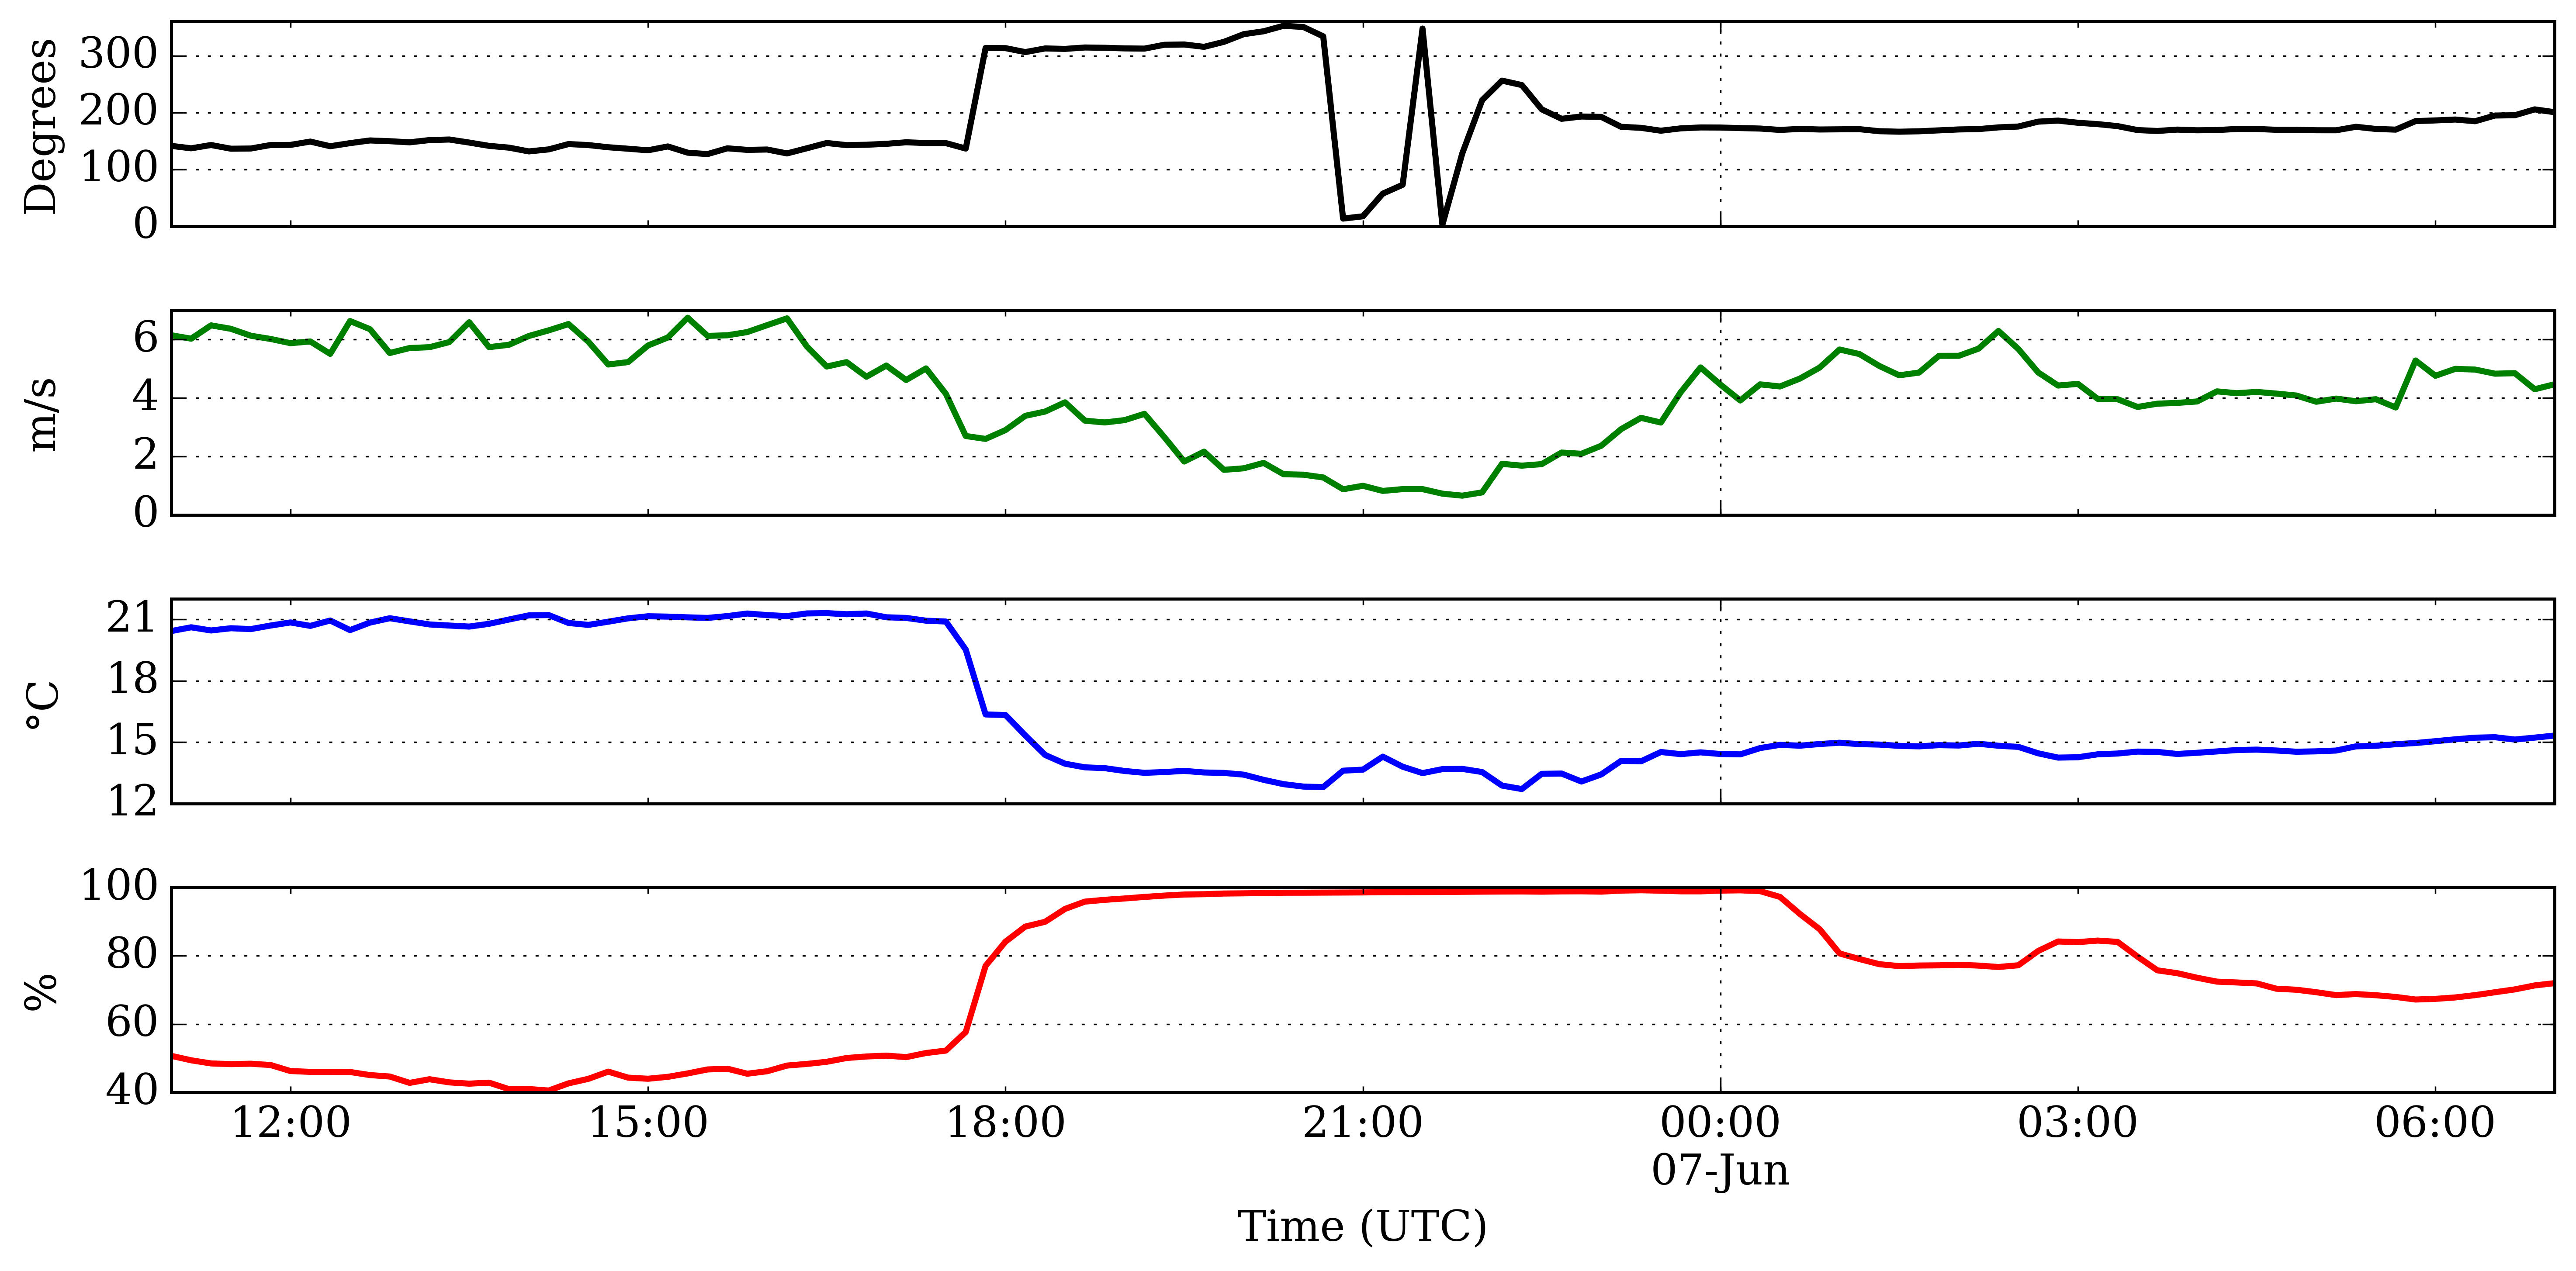
\includegraphics[width=1.0\textwidth]{graphics/results/balcony-addendum/balcony_front_mast.png}
    \caption{Mast measurements during a passing cold front at {\O}sterild test center on June 6-7, 2016.
    Top panel: Wind direction at 40 m AGL. Second panel: Wind speed at 40 m AGL. Third panel: Temperature at 37 m AGL. Bottom panel: Relative humidity at 7 m AGL}
    \label{fig:balcony-front-mast}
\end{figure}

The event is clearly visible in the lidar observations from the Sirocco unit, shown in Figure \ref{fig:lidar_front_ppis_8up}. The frontal boundary is located where the sign of the radial speeds switch from positive (outflow) to negative (inflow). It is first detected 7 km away from the mast position, and the propagation can be tracked over a 2-hour period as it approaches the test site.

% need to clear page before & after this figure as it's huge!
\clearpage
\begin{figure}[htbp]
    \centering
        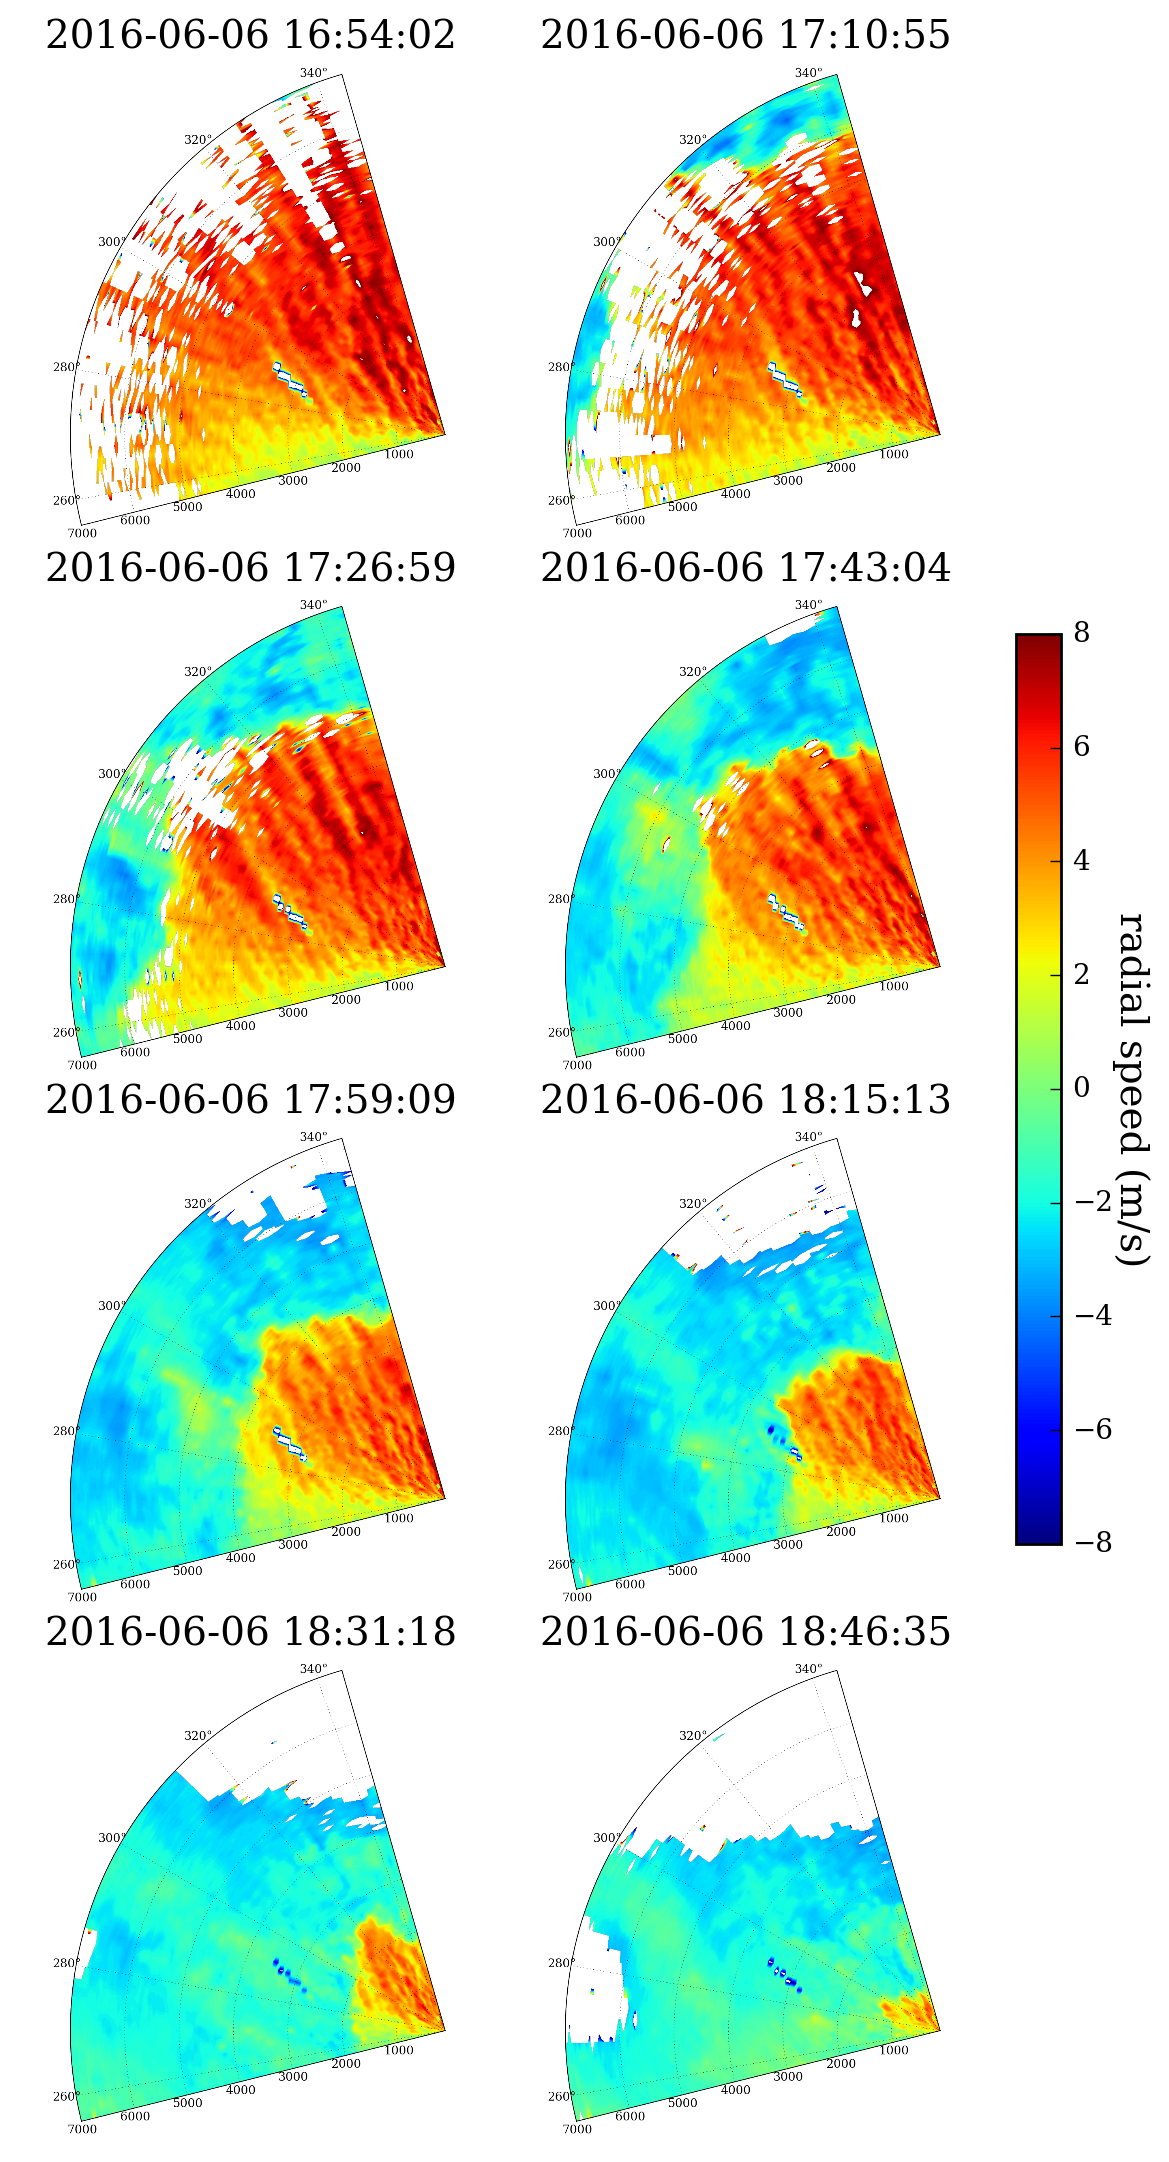
\includegraphics[width=1.0\textwidth, height=1.0\textheight, keepaspectratio]{graphics/results/balcony-addendum/lidar_front_ppis_8up.png}
    \caption{Lidar observations of the frontal passage event from the Sirocco unit. Images are single PPI scans spaced 15-minutes apart. Timestamps are in UTC format}
    \label{fig:lidar_front_ppis_8up}
\end{figure}
\clearpage

This event is an example of a very difficult to forecast phenomenon. Statistical methods including persistence and autoregressive (AR) models will fail spectacularly as there is no connection between the recent past and impending conditions. While physical approaches including numerical weather prediction (NWP) models are in many cases able to predict the existence of a passing weather front, correctly predicting the precise timing is notoriously difficult (phase error).

To further examine the usefulness of the upwind lidar system in capturing the event, predictions from an NWP model were compared with the local site measurements. 
Weather Research and Forecasting (WRF) version 3.5.1 model outputs at 2 km spatial resolution and 1 hour temporal resolution were obtained from Andrea Hahmann at DTU Wind Energy. The domain is shown in Figure \ref{fig:wrf_grid_annotated} along with the grid cell nearest to the met-mast. The distance from the met-mast position to the nearest grid cell is 1.16 km.

\begin{figure}[htbp]
    \centering
        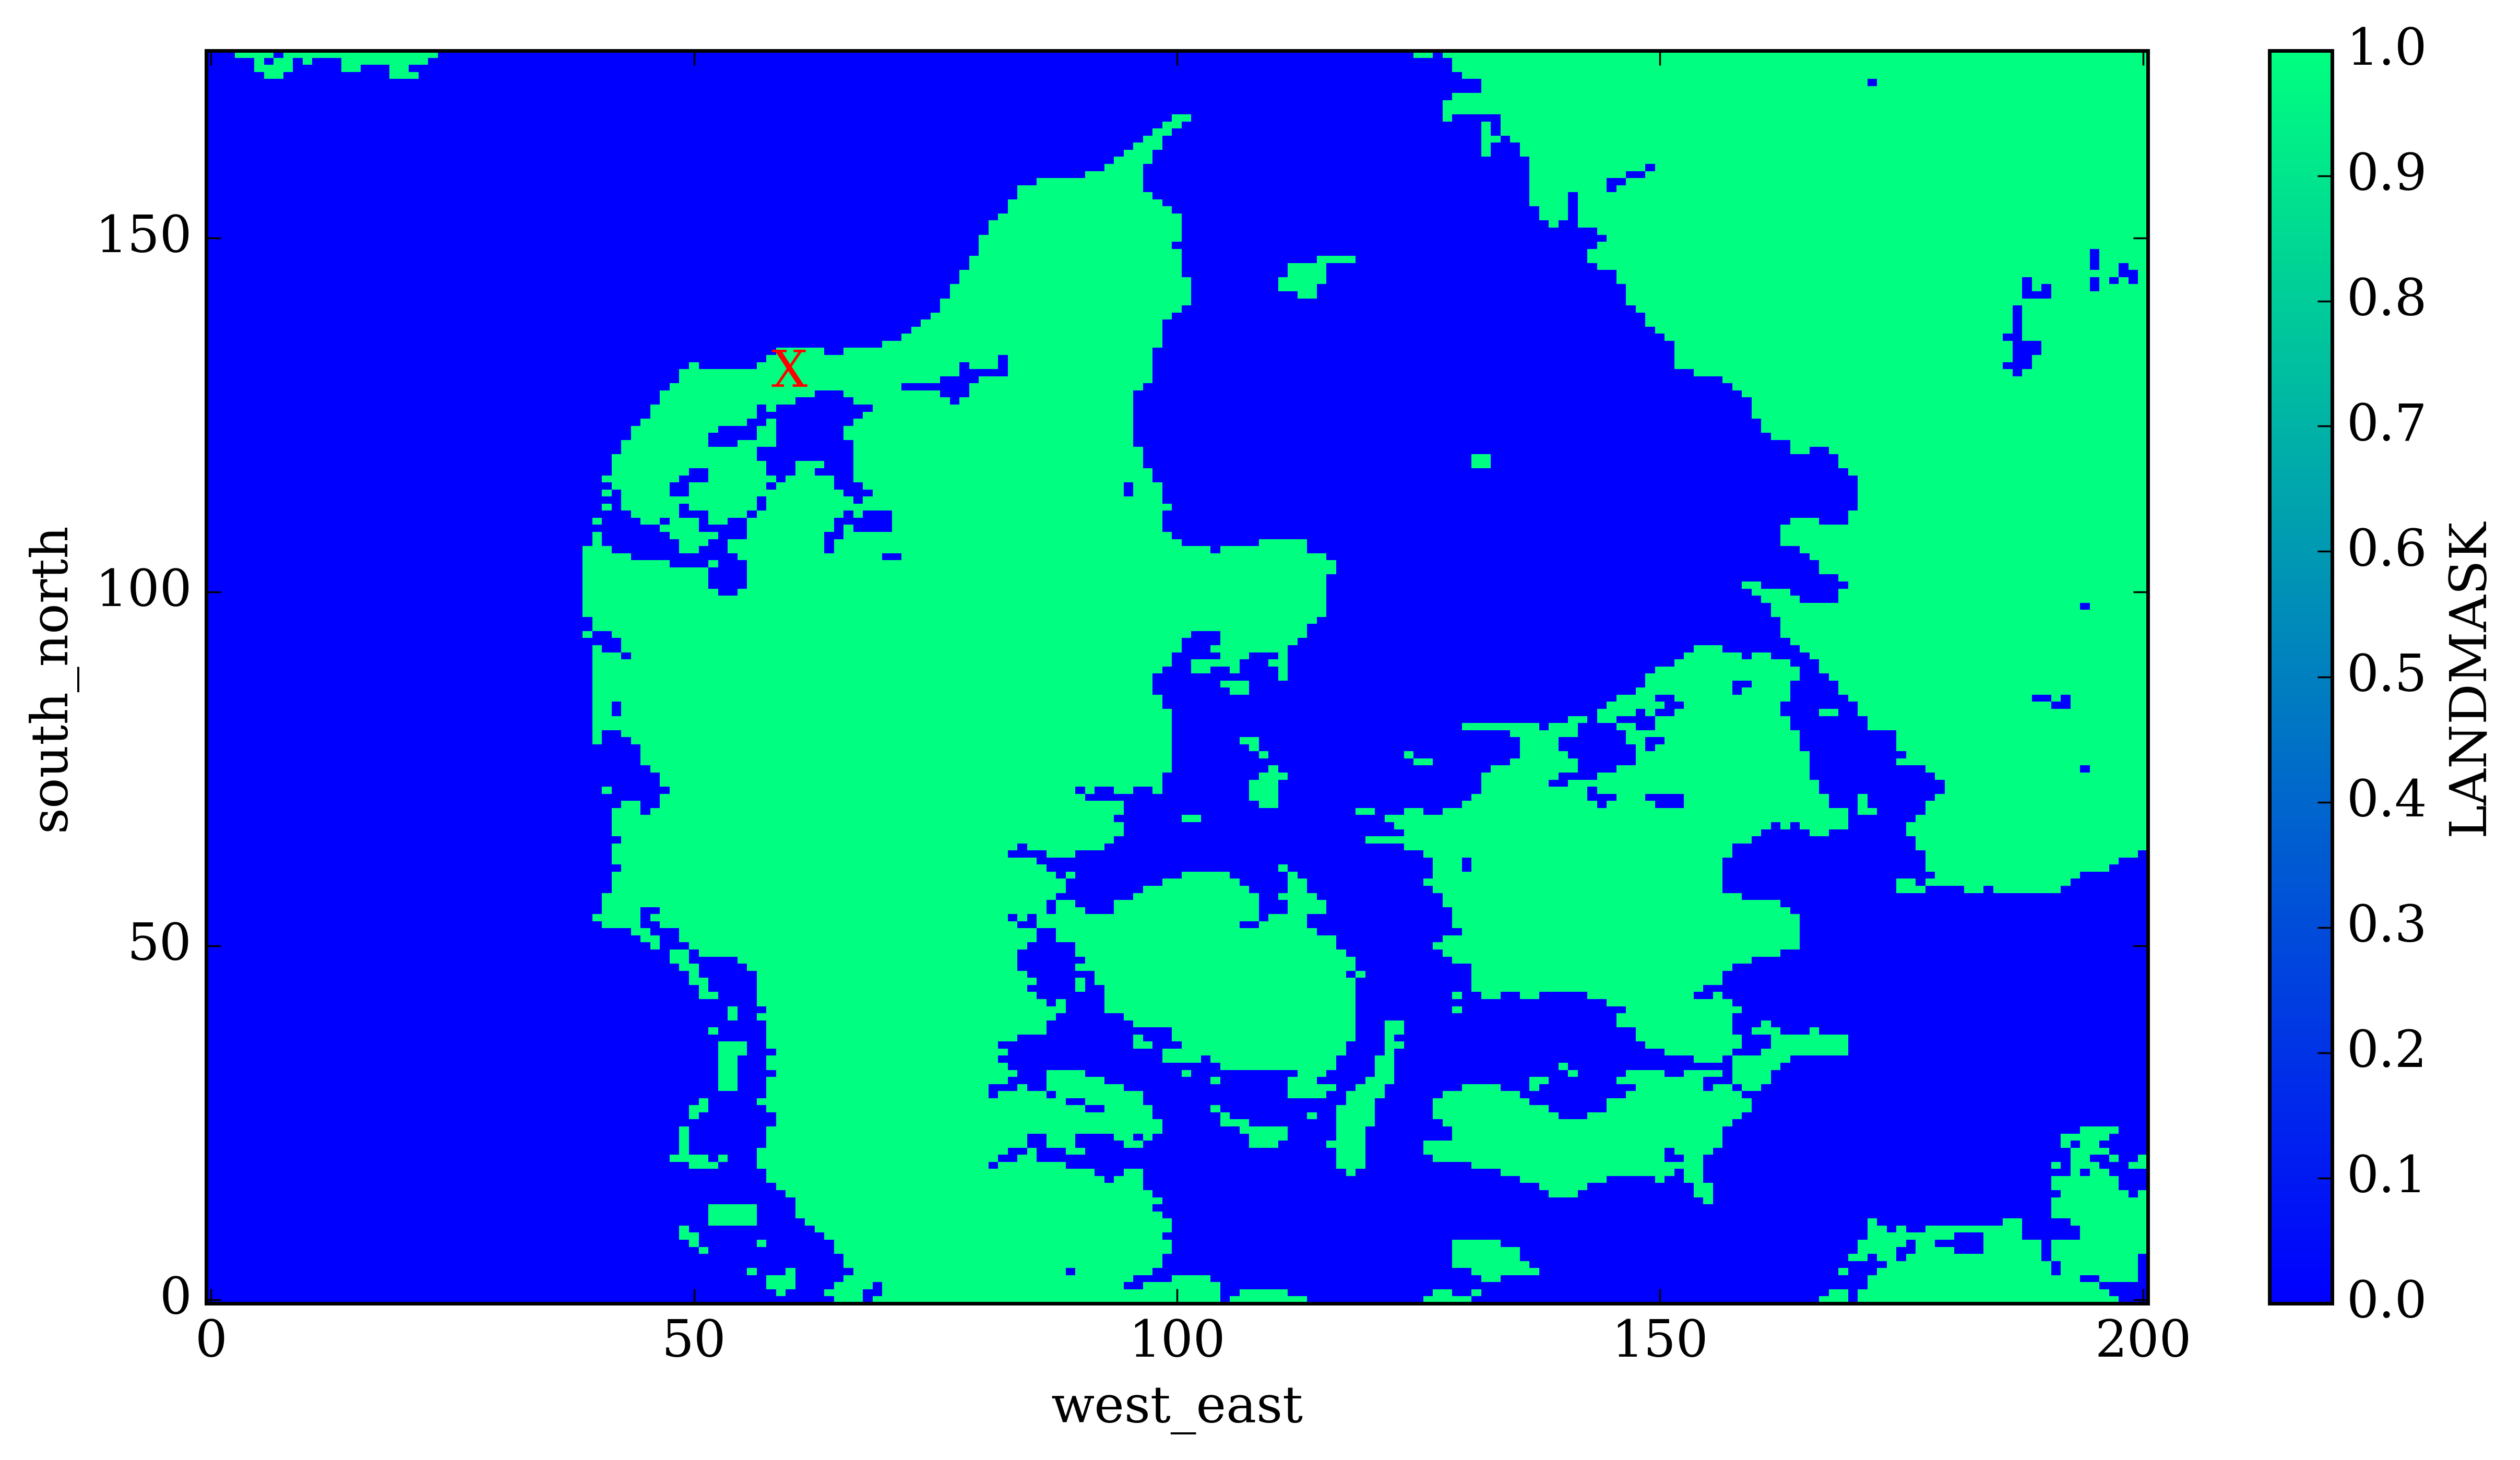
\includegraphics[width=0.75\textwidth]{graphics/results/balcony-addendum/wrf_grid_annotated.png}
    \caption{Domain for WRF simulation, with a red X denoting the chosen grid cell nearest to the met-mast}
    \label{fig:wrf_grid_annotated}
\end{figure}

Four runs: two initialized on June 5th at 0Z (midnight UTC) and 12Z (noon UTC), and two initialized on June 6th (0Z and 12Z) were used to make comparisons between wind speed and direction predictions and the reference site measurements. The met-mast measurements have been converted to UTC time for synchronization with the WRF model outputs.

\begin{figure}[H]
    \centering
        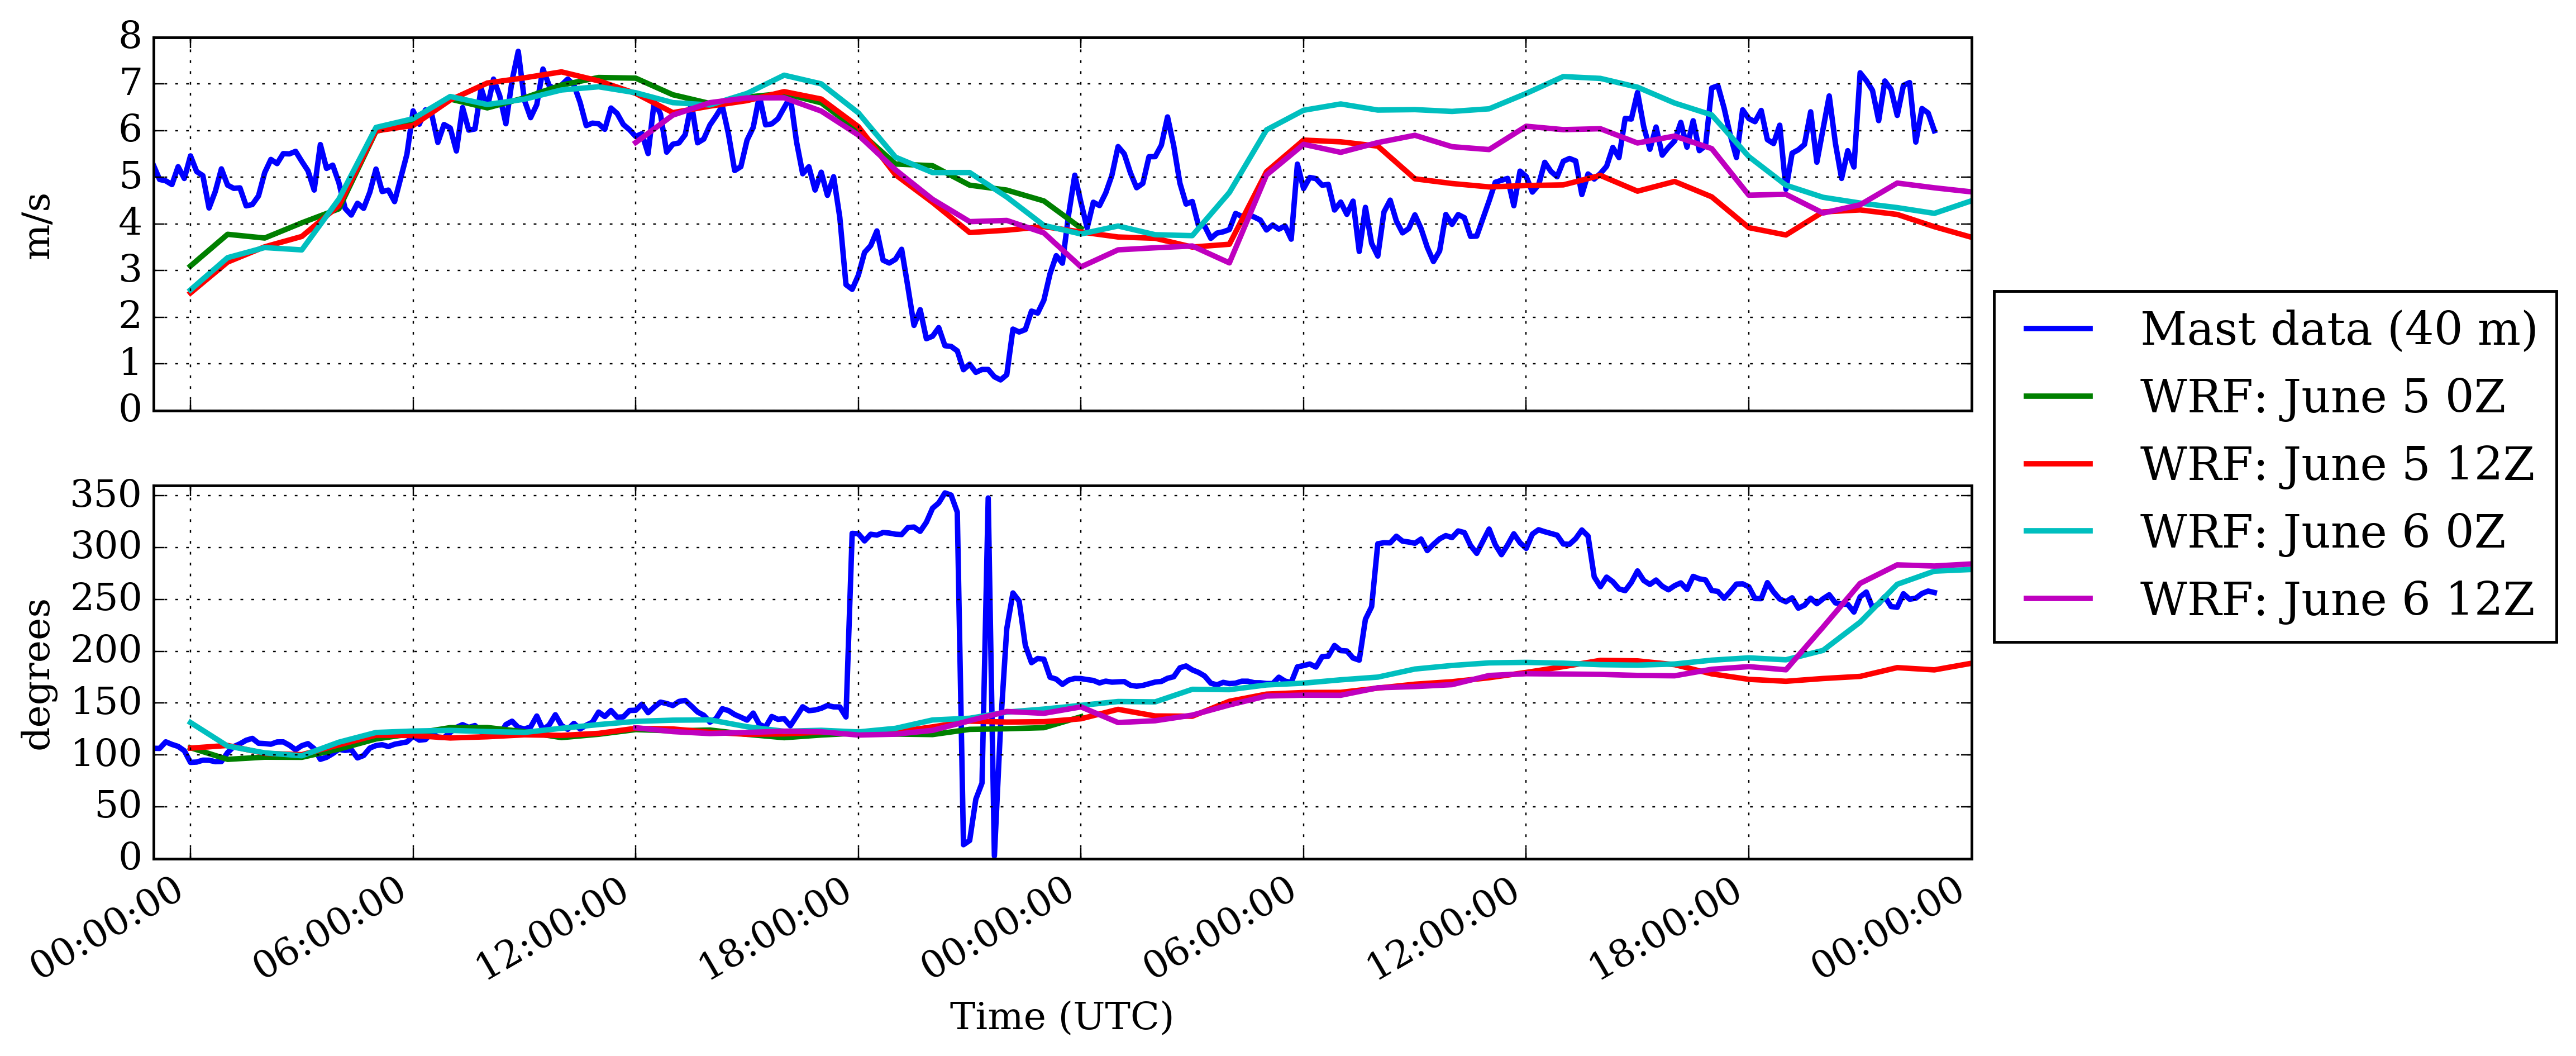
\includegraphics[width=1.0\textwidth]{graphics/results/balcony-addendum/wrf_mast_comparison.png}
    \caption{Comparison of four WRF model predictions with reference met-mast measurements}
    \label{fig:wrf_mast_comparison}
\end{figure}

WRF results are largely consistent across the four runs. Predictions between midnight and 6 PM UTC appropriately match the observational data from the met-mast. However, after this time the forecast does not capture the direction change which is a result of the event observed by the lidar. A further example of a timing (phase) error can be seen in the second direction veer occurring at 8 AM but forecasted to occur 12 hours later.

In summary, the lidar observations have demonstrated a clear value in capturing and tracking a weather event of potential concern as it approaches a wind turbine or wind farm. The event was not predicted by the WRF NWP approach, but was detected 2 hours beforehand by the scanning lidar and its propagation was tracked until arriving to the met-mast position.

This result supports the use of upwind lidar data for detecting and forecasting the arrival of large scale events at a local site. Particularly for sites with recurring localized weather patterns, this application carries promise when used as a classification and warning system to the operator or automated control systems.

%--------------------------------------------------------------------------------
\clearpage
\section{Addendum 2: Key results and lessons learned}
\label{sec:balcony_addendum2}

\begin{itemize}
    \item Ideal measurement setup
    \item Upwind space-time correlations investigated
    \item Comparison of average advection behavior between theoretical (Taylor's frozen turbulence hypothesis) and empirical (lidar retrieved winds)
    \item Simple wind retrieval method demonstrated which works well for wind speed but less favorably for wind direction
    \item Lidar based minute-scale wind speed forecast model implemented which can operate in real-time
    \item Rolling training and prediction approach used which assimilates the last observations to update model weights
    \item RMSE errors reduced by XXXX compared to persistence of 10-minute moving average
    \item Short gust event detected and tracked over 15-minute time period
    
    \item Weather event captured and tracked with a lead time of 2-hours which was not forecasted to occur by NWP models.
    
\end{itemize}

%--------------------------------------------------------------------------------
\clearpage
\section{Introduction to third study: LASCAR experiment}
\label{sec:lascar_intro}

Placeholder

The data set and campaign metadata have been published on DTU's data repository (\cite{lascar_dataset}).

%--------------------------------------------------------------------------------
\clearpage
\section{Minute-Scale Wind Vector Forecasting Using Scanning Lidar Inputs to a Convolutional LSTM Neural Network}
\label{sec:lascar_paper}

Placeholder for LASCAR paper
%\includepdf[pages=-]{papers/LASCAR_paper.pdf}

%--------------------------------------------------------------------------------
\clearpage
\section{Addendum: Key results and lessons learned}
\label{sec:lascar_addendum}

Placeholder